% !TeX spellcheck = en-US
% !TeX encoding = utf8
% !TeX program = lualatex
% !BIB program = biber
% -*- coding:utf-8 mod:LaTeX -*-


% vv  scroll down to line 200 for content  vv


\let\ifdeutsch\iffalse
\let\ifenglisch\iftrue
% EN: This file is loaded before the \documentclass command in the main document

% EN: The following package allows \\ at the title page
%     For more information see https://github.com/latextemplates/scientific-thesis-cover/issues/4
\RequirePackage{kvoptions-patch}

\ifenglisch
  \PassOptionsToClass{numbers=noenddot}{scrbook}
\else
  %()Aus scrguide.pdf - der Dokumentation von KOMA-Script)
  %Nach DUDEN steht in Gliederungen, in denen ausschließlich arabische Ziffern für die Nummerierung
  %verwendet werden, am Ende der Gliederungsnummern kein abschließender Punkt
  %(siehe [DUD96, R3]). Wird hingegen innerhalb der Gliederung auch mit römischen Zahlen
  %oder Groß- oder Kleinbuchstaben gearbeitet, so steht am Ende aller Gliederungsnummern ein
  %abschließender Punkt (siehe [DUD96, R4])
  \PassOptionsToClass{numbers=autoendperiod}{scrbook}
\fi

% Warns about outdated packages and missing caption declarations
% See https://www.ctan.org/pkg/nag
\RequirePackage[l2tabu, orthodox]{nag}

%DE: Neue deutsche Trennmuster
%    Siehe http://www.ctan.org/pkg/dehyph-exptl und http://projekte.dante.de/Trennmuster/WebHome
%    Nur für pdflatex, nicht für lualatex
\RequirePackage{ifluatex}
\ifluatex
  % do not load anything
\else
  \ifdeutsch
    \RequirePackage[ngerman=ngerman-x-latest]{hyphsubst}
  \fi
\fi

\documentclass[
  % fontsize=11pt is the standard
  a4paper,  % Standard format - only KOMAScript uses paper=a4 - https://tex.stackexchange.com/a/61044/9075
  twoside,  % we are optimizing for both screen and two-side printing. So the page numbers will jump, but the content is configured to stay in the middle (by using the geometry package)
  bibliography=totoc,
  %               idxtotoc,   %Index ins Inhaltsverzeichnis
  %               liststotoc, %List of X ins Inhaltsverzeichnis, mit liststotocnumbered werden die Abbildungsverzeichnisse nummeriert
  headsepline,
  cleardoublepage=empty,
  parskip=half,
  %               draft    % um zu sehen, wo noch nachgebessert werden muss - wichtig, da Bindungskorrektur mit drin
  draft=false
]{scrbook}
% !TeX encoding = utf8
% -*- coding:utf-8 mod:LaTeX -*-

% EN: This file includes basic packages and sets options. The order of package
%     loading is important

% DE: In dieser Datei werden zuerst die benoetigten Pakete eingebunden und
%     danach diverse Optionen gesetzt. Achtung Reihenfolge ist entscheidend!


% EN: Styleguide:
% - English comments are prefixed with "EN", German comments are prefixed with "DE"
% - Prefixed headings define the language for the subsequent paragraphs
% - It is tried to organize packages in blocks. Bocks are separated by two empty lines.

% DE: Styleguide:
%
% Ein sehr kleiner Styleguide. Packages werden in Blöcken organisiert.
% Zwischen zwei Blöcken sind 2 Leerzeilen!


% EN: Enable copy and paste of text from the PDF
%     Only required for pdflatex. It "just works" in the case of lualatex.
%     mmap enables mathematical symbols, but does not work with the newtx font set
%     See: https://tex.stackexchange.com/a/64457/9075
%     Other solutions outlined at http://goemonx.blogspot.de/2012/01/pdflatex-ligaturen-und-copynpaste.html and http://tex.stackexchange.com/questions/4397/make-ligatures-in-linux-libertine-copyable-and-searchable
%     Trouble shooting outlined at https://tex.stackexchange.com/a/100618/9075

\ifluatex
\else
  \usepackage{cmap}
\fi


% EN: File encoding
% DE: Codierung
%     Wir sind im 21 Jahrhundert, utf-8 löst so viele Probleme.
%
% Mit UTF-8 funktionieren folgende Pakete nicht mehr. Bitte beachten!
%   * fancyvrb mit §
%   * easylist -> http://www.ctan.org/tex-archive/macros/latex/contrib/easylist/
\ifluatex
  % EN: See https://tex.stackexchange.com/a/158517/9075
  %     Not required, because of usage of fontspec package
  %\usepackage[utf8]{luainputenc}
\else
  \usepackage[utf8]{inputenc}
\fi


% DE: Parallelbetrieb tex4ht und pdflatex

\makeatletter
\@ifpackageloaded{tex4ht}{
  \def\iftex4ht{\iftrue}
}{
  \def\iftex4ht{\iffalse}
}
\makeatother


% EN: Mathematics
% DE: Mathematik
%
% DE: Viele Mathematik-Sachen. Siehe https://texdoc.net/pkg/amsmath
%
% EN: Options must be passed this way, otherwise it does not work with glossaries
% DE: fleqn (=Gleichungen linksbündig platzieren) funktioniert nicht direkt. Es muss noch ein Patch gemacht werden:
\PassOptionsToPackage{leqno}{amsmath}
%
% DE: amsmath Muss nicht mehr geladen werden, da es von newtxmath automatisch geladen wird
% \usepackage{amsmath}


%% EN: Fonts
%% DE: Schriften
%%
%% !!! If you change the font, be sure that words such as "workflow" can
%% !!! still be copied from the PDF. If this is not the case, you have
%% !!! to use glyphtounicode. See comment at cmap package


% EN: Times Roman for all text
\ifluatex
  % source: Second proposed fix from the following answer: https://tex.stackexchange.com/a/394137
  \usepackage[no-math]{fontspec}
  \setmainfont{TeXGyreTermes-Regular}[
       BoldFont       = TeXGyreTermes-Bold ,
       ItalicFont     = TeXGyreTermes-Italic ,
       BoldItalicFont = TeXGyreTermes-BoldItalic,
       NFSSFamily     = ntxtlf]
  \setsansfont{TeX Gyre Heros Regular}[
       Scale=.9,
       BoldFont       = TeX Gyre Heros Bold,
       ItalicFont     = TeX Gyre Heros Italic,
       BoldItalicFont = TeX Gyre Heros BoldItalic]
  \setmonofont[StylisticSet={1,3},Scale=.9]{inconsolata}
  \RequirePackage{newtxmath}
\else
  \RequirePackage{newtxtext}
  \RequirePackage{newtxmath}
  % EN: looks good with times, but no equivalent for lualatex found,
  %     therefore replaced with inconsolata
  %\RequirePackage[zerostyle=b,scaled=.9]{newtxtt}
  \RequirePackage[varl,scaled=.9]{inconsolata}
\fi

% EN: Fallback font - if the subsequent font packages do not define a font (e.g., monospaced)
%     This is the modern package for "Computer Modern".
%     In case this gets activated, one has to switch from cmap package to glyphtounicode (in the case of pdflatex)
% DE: Fallback-Schriftart
%\usepackage[%
%    rm={oldstyle=false,proportional=true},%
%    sf={oldstyle=false,proportional=true},%
%    tt={oldstyle=false,proportional=true,variable=true},%
%    qt=false%
%]{cfr-lm}

% EN: Headings are typset in Helvetica (which is similar to Arial)
% DE: Schriftart fuer die Ueberschriften - ueberschreibt lmodern
%\usepackage[scaled=.95]{helvet}

% DE: Für Schreibschrift würde tun, muss aber nicht
%\usepackage{mathrsfs} %  \mathscr{ABC}

% EN: Font for the main text
% DE: Schriftart fuer den Fliesstext - ueberschreibt lmodern
%     Linux Libertine, siehe http://www.linuxlibertine.org/
%     Packageparamter [osf] = Minuskel-Ziffern
%     rm = libertine im Brottext, Linux Biolinum NICHT als serifenlose Schrift, sondern helvet (von oben) beibehalten
%\usepackage[rm]{libertine}

% EN: Alternative Font: Palantino. It is recommeded by Prof. Ludewig for German texts
% DE: Alternative Schriftart: Palantino, Packageparamter [osf] = Minuskel-Ziffern
%     Bitte nur in deutschen Texten
%\usepackage{mathpazo} %ftp://ftp.dante.de/tex-archive/fonts/mathpazo/ - Tipp aus DE-TEX-FAQ 8.2.1

% DE: Schriftart fuer Programmcode - ueberschreibt lmodern
%     Falls auskommentiert, wird die Standardschriftart lmodern genommen
%     Fuer schreibmaschinenartige Schluesselwoerter in den Listings - geht bei alten Installationen nicht, da einige Fontshapes (<>=) fehlen
%\usepackage[scaled=.92]{luximono}
%\usepackage{courier}
% DE: BeraMono als Typewriter-Schrift, Tipp von http://tex.stackexchange.com/a/71346/9075
%\usepackage[scaled=0.83]{beramono}

% EN: backticks (`) are rendered as such in verbatim environments.
%     See following links for details:
%     - https://tex.stackexchange.com/a/341057/9075
%     - https://tex.stackexchange.com/a/47451/9075
%     - https://tex.stackexchange.com/a/166791/9075
\usepackage{upquote}

% DE: Symbole
%
%\usepackage[geometry]{ifsym} % \BigSquare
%\usepackage{mathabx}
%\usepackage{stmaryrd} %fuer \ovee, \owedge, \otimes
%\usepackage{marvosym} %fuer \Writinghand %patched to not redefine \Rightarrow
%\usepackage{mathrsfs} %mittels \mathscr{} schoenen geschwungenen Buchstaben erzeugen
%\usepackage{calrsfs} %\mathcal{} ein bisserl dickeren buchstaben erzeugen - sieht net so gut aus.
%durch mathpazo ist das schon definiert

%
%\usepackage{amssymb}

% EN: For \texttrademark{}
\usepackage{textcomp}

% EN: name-clashes von marvosym und mathabx vermeiden:
\def\delsym#1{%
  %  \expandafter\let\expandafter\origsym\expandafter=\csname#1\endcsname
  %  \expandafter\let\csname orig#1\endcsname=\origsym
  \expandafter\let\csname#1\endcsname=\relax
}

%\usepackage{pifont}
%\usepackage{bbding}
%\delsym{Asterisk}
%\delsym{Sun}\delsym{Mercury}\delsym{Venus}\delsym{Earth}\delsym{Mars}
%\delsym{Jupiter}\delsym{Saturn}\delsym{Uranus}\delsym{Neptune}
%\delsym{Pluto}\delsym{Aries}\delsym{Taurus}\delsym{Gemini}
%\delsym{Rightarrow}
%\usepackage{mathabx} - Ueberschreibt leider zu viel - und die \le-Zeichen usw. sehen nicht gut aus!


% EN: Modern font encoding
%     Has to be loaded AFTER any font packages. See https://tex.stackexchange.com/a/2869/9075.
\ifluatex
\else
  \usepackage[T1]{fontenc}
\fi
%


% EN: Character protrusion and font expansion. See http://www.ctan.org/tex-archive/macros/latex/contrib/microtype/
% DE: Optischer Randausgleich und Grauwertkorrektur

\usepackage[
  babel=true, % EN: Enable language-specific kerning. Take language-settings from the languge of the current document (see Section 6 of microtype.pdf)
  expansion=alltext,
  protrusion=alltext-nott, % EN: Ensure that at listings, there is no change at the margin of the listing
  final % EN: Always enable microtype, even if in draft mode. This helps finding bad boxes quickly.
        %     In the standard configuration, this template is always in the final mode, so this option only makes a difference if "pros" use the draft mode
]{microtype}


% EN: \texttt{test -- test} keeps the "--" as "--" (and does not convert it to an en dash)
\DisableLigatures{encoding = T1, family = tt* }

% DE: fuer microtype
% DE: tracking=true muss als Parameter des microtype-packages mitgegeben werden
% DE: Deaktiviert, da dies bei Algorithmen seltsam aussieht

%\DeclareMicrotypeSet*[tracking]{my}{ font = */*/*/sc/* }%
%\SetTracking{ encoding = *, shape = sc }{ 45 }
% DE: Hier wird festgelegt,
%     dass alle Passagen in Kapitälchen automatisch leicht
%     gesperrt werden.
%     Quelle: http://homepage.ruhr-uni-bochum.de/Georg.Verweyen/pakete.html
%    Deaktiviert, da sonst "BPEL", "BPMN" usw. wirklich komisch aussehen.
%     Macht wohl nur bei geisteswissenschaftlichen Arbeiten Sinn.


% EN: amsmath teaks


% EN: Fixes bugs in AMS math
%     Corrently conflicts with unicode-math
% \usepackage{mathtools}

%\numberwithin{equation}{section}
%\renewcommand{\theequation}{\thesection.\Roman{equation}}

% EN: work-around ams-math problem with align and 9 -> 10. Does not work with glossaries, No visual changes.
%\addtolength\mathindent{1em}


% EN: For theorems, replacement for amsthm
\usepackage[amsmath,hyperref]{ntheorem}
\theorempreskipamount 2ex plus1ex minus0.5ex
\theorempostskipamount 2ex plus1ex minus0.5ex
\theoremstyle{break}
\newtheorem{definition}{Definition}[section]


% CTAN: https://ctan.org/pkg/lccaps
% Doc: http://texdoc.net/pkg/lccaps
%
% Required for DE/EN \initialism
\usepackage{lccaps}


% EN: Defintion of colors. Argument "hyperref" is not used as we do not want to change border colors of links: Links are not colored anymore.
% DE: Farbdefinitionen
\usepackage[dvipsnames]{xcolor}


% EN: Required for custom acronyms/glossaries style.
%     Left aligned Columns in tables with fixed width.
%     See http://tex.stackexchange.com/questions/91566/syntax-similar-to-centering-for-right-and-left
\usepackage{ragged2e}


% DE: Wichtig, ansonsten erscheint "No room for a new \write"
\usepackage{scrwfile}


% EN: Support for language-specific hyphenation
% DE: Neue deutsche Rechtschreibung und Literatur statt "Literature"
%     Die folgende Einstellung ist der Nachfolger von ngerman.sty
\ifdeutsch
  % DE: letzte Sprache ist default, Einbindung von "american" ermöglicht \begin{otherlanguage}{amercian}...\end{otherlanguage} oder \foreignlanguage{american}{Text in American}
  %     Siehe auch http://tex.stackexchange.com/a/50638/9075
  \usepackage[american,main=ngerman]{babel}
  % Ein "abstract" ist eine "Kurzfassung", keine "Zusammenfassung"
  \addto\captionsngerman{%
    \renewcommand\abstractname{Kurzfassung}%
  }
  \ifluatex
    % EN: conditionally disable ligatures. See https://github.com/latextemplates/scientific-thesis-template/issues/54
    %     for a discussion
    \usepackage[ngerman]{selnolig}
  \fi
\else
  % EN: Set English as language and allow to write hyphenated"=words
  %     `american`, `english` and `USenglish` are synonyms for babel package (according to https://tex.stackexchange.com/questions/12775/babel-english-american-usenglish).
  %      "english" has to go last to set it as default language
  \usepackage[ngerman,main=english]{babel}
  % EN: Hint by http://tex.stackexchange.com/a/321066/9075 -> enable "= as dashes
  \addto\extrasenglish{\languageshorthands{ngerman}\useshorthands{"}}
  \ifluatex
    % EN: conditionally disable ligatures. See https://github.com/latextemplates/scientific-thesis-template/issues/54
    %     for a discussion
    \usepackage[english]{selnolig}
  \fi
\fi
%


% EN: For easy quotations: \enquote{text}
%     This package is very smart when nesting is applied, otherwise textcmds (see below) provides a shorter command
%     Note that this package results in a warning when it is loaded before minted (actually fvextra).
% DE: Anführungszeichen
%     Zitate in \enquote{...} setzen, dann werden automatisch die richtigen Anführungszeichen verwendet.
%     Dieses package erzeugt eine Warnung, wenn es vor minted (genauer fvextra) geladen wird.
\usepackage{csquotes}


% EN: For even easier quotations: \qq{text}.
%     Is not smart in the case of nesting, but good enough for the most cases
\usepackage{textcmds}
\ifdeutsch
  % EN: German quotes are different. So do not use the English quotes, but the ones provided by the csquotes package.
  \renewcommand{\qq}[1]{\enquote{#1}}
\fi


% EN: extended enumarations
% DE: erweitertes Enumerate
\usepackage{paralist}


% DE: Gestaltung der Kopf- und Fußteilen

\usepackage[automark]{scrlayer-scrpage}

\automark[section]{chapter}
\setkomafont{pageheadfoot}{\normalfont\sffamily}
\setkomafont{pagenumber}{\normalfont\sffamily}

% DE: funktioniert nicht: Alle Linien sind hier weg
%\setheadsepline[.4pt]{.4pt}


% DE: Intelligentes Leerzeichen um hinter Abkürzungen die richtigen Abstände zu erhalten, auch leere.
%     Siehe commands.tex \gq{}
\usepackage{xspace}
% DE: Macht \xspace und \enquote kompatibel
\makeatletter
\xspaceaddexceptions{\grqq \grq \csq@qclose@i \} }
\makeatother


\newcommand{\eg}{e.\,g.,\ }
\newcommand{\ie}{i.\,e.,\ }


% EN: introduce \powerset - hint by http://matheplanet.com/matheplanet/nuke/html/viewtopic.php?topic=136492&post_id=997377
\DeclareFontFamily{U}{MnSymbolC}{}
\DeclareSymbolFont{MnSyC}{U}{MnSymbolC}{m}{n}
\DeclareFontShape{U}{MnSymbolC}{m}{n}{
  <-6>    MnSymbolC5
  <6-7>   MnSymbolC6
  <7-8>   MnSymbolC7
  <8-9>   MnSymbolC8
  <9-10>  MnSymbolC9
  <10-12> MnSymbolC10
  <12->   MnSymbolC12%
}{}
\DeclareMathSymbol{\powerset}{\mathord}{MnSyC}{180}


% EN: Package for the appendix
% DE: Anhang
\usepackage{appendix}
%[toc,page,title,header]
%


% EN: Graphics
% DE: Grafikeinbindungen
%
% EN: The parameter "pdftex" is not required
\usepackage{graphicx}
\graphicspath{{\getgraphicspath}}
\newcommand{\getgraphicspath}{graphics/}


% EN: Enables inclusion of SVG graphics - 1:1 approach
%    This is NOT the approach of https://ctan.org/pkg/svg-inkscape,
%     which allows text in SVG to be typeset using LaTeX
%     We just include the SVG as is.
\usepackage{epstopdf}
\epstopdfDeclareGraphicsRule{.svg}{pdf}{.pdf}{%
  inkscape -z -D --file=#1 --export-pdf=\OutputFile
}


% EN: Enables inclusion of SVG graphics - text-rendered-with-LaTeX-approach
%     This is the approach of https://ctan.org/pkg/svg-inkscape,
\newcommand{\executeiffilenewer}[3]{%
  \IfFileExists{#2}
  {
    %\message{file #2 exists}
    \ifnum\pdfstrcmp{\pdffilemoddate{#1}}%
      {\pdffilemoddate{#2}}>0%
      {\immediate\write18{#3}}
    \else
      {%\message{file up to date #2}
      }
    \fi%
  }{
    %\message{file #2 doesn't exist}
    %\message{argument: #3}
    %\immediate\write18{echo "test" > xoutput.txt}
    \immediate\write18{#3}
  }
}
\newcommand{\includesvg}[1]{%
  \executeiffilenewer{#1.svg}{#1.pdf}%
  {
    inkscape -z -D --file=\getgraphicspath#1.svg %
    --export-pdf=\getgraphicspath#1.pdf --export-latex}%
  \input{\getgraphicspath#1.pdf_tex}%
}


% EN: Enable typesetting values with SI units.
\ifdeutsch
  \usepackage[mode=text,group-four-digits]{siunitx}
  \sisetup{locale=DE}
\else
  \usepackage[mode=text,group-four-digits,group-separator={,}]{siunitx}
  \sisetup{locale=US}
\fi


% EN: Extensions for tables
% DE: Tabellenerweiterungen
\usepackage{array} %increases tex's buffer size and enables ``>'' in tablespecs
\usepackage{longtable}
\usepackage{dcolumn} %Aligning numbers by decimal points in table columns
\ifdeutsch
  \newcolumntype{d}[1]{D{.}{,}{#1}}
\else
  \newcolumntype{d}[1]{D{.}{.}{#1}}
\fi
\setlength{\extrarowheight}{1pt}


% DE: Eine Zelle, die sich über mehrere Zeilen erstreckt.
%     Siehe Beispieltabelle in Kapitel 2
\usepackage{multirow}


% DE: Fuer Tabellen mit Variablen Spaltenbreiten
%\usepackage{tabularx}
%\usepackage{tabulary}


% EN: Links behave as they should. Enables "\url{...}" for URL typesettings.
%     Allow URL breaks also at a hyphen, even though it might be confusing: Is the "-" part of the address or just a hyphen?
%     See https://tex.stackexchange.com/a/3034/9075.
% DE: Links verhalten sich so, wie sie sollen
%     Zeilenumbrüche bei URLs auch bei Bindestrichen erlauben, auch wenn es verwirrend sein könnte: Gehört der Bindestrich zur URL oder ist es ein Trennstrich?
%     Siehe https://tex.stackexchange.com/a/3034/9075.
\usepackage[hyphens]{url}
%
%  EN: When activated, use text font as url font, not the monospaced one.
%      For all options see https://tex.stackexchange.com/a/261435/9075.
% \urlstyle{same}
%
% EN: Hint by http://tex.stackexchange.com/a/10419/9075.
\makeatletter
\g@addto@macro{\UrlBreaks}{\UrlOrds}
\makeatother


% DE: Index über Begriffe, Abkürzungen
%\usepackage{makeidx} makeidx ist out -> http://xindy.sf.net verwenden


% DE: lustiger Hack fuer das Abkuerzungsverzeichnis
%     nach latex durchlauf folgendes ausfuehren
%     makeindex ausarbeitung.nlo -s nomencl.ist -o ausarbeitung.nls
%     danach nochmal latex
%\usepackage{nomencl}
%    \let\abk\nomenclature %Deutsche Ueberschrift setzen
%          \renewcommand{\nomname}{List of Abbreviations}
%        %Punkte zw. Abkuerzung und Erklaerung
%          \setlength{\nomlabelwidth}{.2\hsize}
%          \renewcommand{\nomlabel}[1]{#1 \dotfill}
%        %Zeilenabstaende verkleinern
%          \setlength{\nomitemsep}{-\parsep}
%    \makenomenclature


% EN: Logic for TeX - enables if-then-else in commands
% DE: Logik für TeX
%     FÜr if-then-else @ commands.tex
\usepackage{ifthen}


% EN: Code Listings
% DE: Listings
\usepackage{listings}
\lstset{language=XML,
  showstringspaces=false,
  extendedchars=true,
  basicstyle=\footnotesize\ttfamily,
  commentstyle=\slshape,
  % DE: Original: \rmfamily, damit werden die Strings im Quellcode hervorgehoben. Zusaetzlich evtl.: \scshape oder \rmfamily durch \ttfamily ersetzen. Dann sieht's aus, wie bei fancyvrb
  stringstyle=\ttfamily,
  breaklines=true,
  breakatwhitespace=true,
  % EN: alternative: fixed
  columns=flexible,
  numbers=left,
  numberstyle=\tiny,
  basewidth=.5em,
  xleftmargin=.5cm,
  % aboveskip=0mm, %DE: deaktivieren, falls man lstlistings direkt als floating object benutzt (\begin{lstlisting}[float,...])
  % belowskip=0mm, %DE: deaktivieren, falls man lstlistings direkt als floating object benutzt (\begin{lstlisting}[float,...])
  captionpos=b
}

\ifluatex
\else
  % EN: Enable UTF-8 support - see https://tex.stackexchange.com/q/419327/9075
  \usepackage{listingsutf8}
  \lstset{inputencoding=utf8/latin1}
\fi

\ifdeutsch
  \renewcommand{\lstlistlistingname}{Verzeichnis der Listings}
\fi


% EN: Alternative to listings could be fancyvrb. Can be used together.
% DE: Alternative zu Listings ist fancyvrb. Kann auch beides gleichzeitig benutzt werden.
\usepackage{fancyvrb}
%
% EN: Font size for the normal text
% DE: Groesse fuer den Fliesstext. Falls deaktiviert: \normalsize
%\fvset{fontsize=\small}
%
% DE: Somit kann im Text ganz einfach §verbatim§ text gesetzt werden.
%     Disabled, because UTF-8 does not work any more and lualatex causes issues
%\DefineShortVerb{\§}
%
% EN: Shrink font size of listings
\RecustomVerbatimEnvironment{Verbatim}{Verbatim}{fontsize=\footnotesize}
\RecustomVerbatimCommand{\VerbatimInput}{VerbatimInput}{fontsize=\footnotesize}
%
% EN: Hack for fancyvrb based on http://newsgroups.derkeiler.com/Archive/Comp/comp.text.tex/2008-12/msg00075.html
%     Change of the solution: \Vref somehow collidated with cleveref/varioref as the output of \Vref{} was "Abschnitt 4.3 auf Seite 85"; therefore changed to \myVref -- so completely removed
%     See https://tex.stackexchange.com/q/132420/9075 for more information.
\newcommand{\Vlabel}[1]{\label[line]{#1}\hypertarget{#1}{}}
\newcommand{\lref}[1]{\hyperlink{#1}{\FancyVerbLineautorefname~\ref*{#1}}}


% EN: Tunings of captions for floats, listings, ...
% DE: Bildunterschriften bei floats genauso formatieren wie bei Listings
%     Anpassung wird unten bei den newfloat-Deklarationen vorgenommen
%     https://www.ctan.org/pkg/caption2 is superseeded by this package.
\usepackage{caption}


% EN: Provides rotating figures, where the PDF page is also turned
% DE: Ermoeglicht es, Abbildungen um 90 Grad zu drehen
%     Alternatives Paket: rotating Allerdings wird hier nur das Bild gedreht, während bei lscape auch die PDF-Seite gedreht wird.
%     Das Paket lscape dreht die Seite auch nicht
\usepackage{pdflscape}


% EN: Required for proper environments of fancyvrb and lstlistings
%    There is also the newfloat pacakge (recommended by minted), but we currently have no expericene with that
% DE: Wird für fancyvrb und für lstlistings verwendet
\usepackage{float}
%
% EN: Alternative to float package
%\usepackage{floatrow}
% DE: zustäzlich für den Paramter [H] = Floats WIRKLICH da wo sie deklariert wurden paltzieren - ganz ohne Kompromisse
%     floatrow ist der Nachfolger von float
%     Allerdings macht floatrow in manchen Konstellationen Probleme. Deshalb ist das Paket deaktiviert.
%
% EN: See http://www.tex.ac.uk/cgi-bin/texfaq2html?label=floats
% DE: floats IMMER nach einer Referenzierung platzieren
%\usepackage{flafter}


% EN: Put footnotes below floats
%     Source: https://tex.stackexchange.com/a/32993/9075
\usepackage{stfloats}
\fnbelowfloat


% EN: For nested figures
% DE: Fuer Abbildungen innerhalb von Abbildungen
%     Ersetzt die Pakete subfigure und subfig - siehe https://tex.stackexchange.com/a/13778/9075
\usepackage[hypcap=true]{subcaption}


% EN: Extended support for footnotes
% DE: Fußnoten
%
%\usepackage{dblfnote}  %Zweispaltige Fußnoten
%
% Keine hochgestellten Ziffern in der Fußnote (KOMA-Script-spezifisch):
%\deffootnote[1.5em]{0pt}{1em}{\makebox[1.5em][l]{\bfseries\thefootnotemark}}
%
% Abstand zwischen Fußnoten vergrößern:
%\setlength{\footnotesep}{.85\baselineskip}
%
% EN: Following command disables the separting line of the footnote
% DE: Folgendes Kommando deaktiviert die Trennlinie zur Fußnote
%\renewcommand{\footnoterule}{}
%
\addtolength{\skip\footins}{\baselineskip} % Abstand Text <-> Fußnote
%
% Fußnoten immer ganz unten auf einer \raggedbottom-Seite
% fnpos kommt aus dem yafoot package
\usepackage{fnpos}
\makeFNbelow
\makeFNbottom


% EN: Variable page heights
% DE: Variable Seitenhöhen zulassen
\raggedbottom


% DE: Falls die Seitenzahl bei einer Referenz auf eine Abbildung nur dann angegeben werden soll,
%     falls sich die Abbildung nicht auf der selben Seite befindet...
\iftex4ht
  %tex4ht does not work well with vref, therefore we emulate vref behavior
  \newcommand{\vref}[1]{\ref{#1}}
\else
  \ifdeutsch
    \usepackage[ngerman]{varioref}
  \else
    \usepackage{varioref}
  \fi
\fi


% EN: More beautiful tables if one uses \toprule, \midrule, \bottomrule
% DE: Noch schoenere Tabellen als mit booktabs mit http://www.zvisionwelt.de/downloads.html
\usepackage{booktabs}
%
%\usepackage[section]{placeins}


% EN: Graphs and Automata
%
% TODO: Since version 3.0 (2013-10-01), it supports pdflatex via the auto-pst-pdf package
%       Requires -shell-escape
%\usepackage{gastex}


%\usepackage{multicol}

% DE: kollidiert mit diplomarbeit.sty
%\usepackage{setspace}


% DE: biblatex statt bibtex
\usepackage[
  backend       = biber, %biber does not work with 64x versions alternative: bibtex8
  %minalphanames only works with biber backend
  sortcites     = true,
  bibstyle      = alphabetic,
  citestyle     = alphabetic,
  giveninits    = true,
  useprefix     = false, %"von, van, etc." will be printed, too. See below.
  minnames      = 1,
  minalphanames = 3,
  maxalphanames = 4,
  maxbibnames   = 99,
  maxcitenames  = 2,
  natbib        = true,
  eprint        = true,
  url           = true,
  doi           = true,
  isbn          = true,
  backref       = true]{biblatex}

% enable more breaks at URLs. See https://tex.stackexchange.com/a/134281.
\setcounter{biburllcpenalty}{7000}
\setcounter{biburlucpenalty}{8000}

\bibliography{lib/mt.bib}
%\addbibresource[datatype=bibtex]{bibliography.bib}

%Do not put "vd" in the label, but put it at "\citeauthor"
%Source: http://tex.stackexchange.com/a/30277/9075
\makeatletter
\AtBeginDocument{\toggletrue{blx@useprefix}}
\AtBeginBibliography{\togglefalse{blx@useprefix}}
\makeatother

%Thin spaces between initials
%http://tex.stackexchange.com/a/11083/9075
\renewrobustcmd*{\bibinitdelim}{\,}

%Keep first and last name together in the bibliography
%http://tex.stackexchange.com/a/196192/9075
\renewcommand*\bibnamedelimc{\addnbspace}
\renewcommand*\bibnamedelimd{\addnbspace}

%Replace last "and" by comma in bibliography
%See http://tex.stackexchange.com/a/41532/9075
\AtBeginBibliography{%
  \renewcommand*{\finalnamedelim}{\addcomma\space}%
}

\DefineBibliographyStrings{ngerman}{
  backrefpage  = {zitiert auf S\adddot},
  backrefpages = {zitiert auf S\adddot},
  andothers    = {et\ \addabbrvspace al\adddot},
  %Tipp von http://www.mrunix.de/forums/showthread.php?64665-biblatex-Kann-%DCberschrift-vom-Inhaltsverzeichnis-nicht-%E4ndern&p=293656&viewfull=1#post293656
  bibliography = {Literaturverzeichnis}
}

% EN: enable hyperlinked author names when using \citeauthor
%     source: http://tex.stackexchange.com/a/75916/9075
\DeclareCiteCommand{\citeauthor}
{\boolfalse{citetracker}%
  \boolfalse{pagetracker}%
  \usebibmacro{prenote}}
{\ifciteindex
  {\indexnames{labelname}}
  {}%
  \printtext[bibhyperref]{\printnames{labelname}}}
{\multicitedelim}
{\usebibmacro{postnote}}

% EN: natbib compatibility
%\newcommand{\citep}[1]{\cite{#1}}
%\newcommand{\citet}[1]{\citeauthor{#1} \cite{#1}}
% EN: Beginning of sentence - analogous to cleveref - important for names such as "zur Muehlen"
%\newcommand{\Citep}[1]{\cite{#1}}
%\newcommand{\Citet}[1]{\Citeauthor{#1} \cite{#1}}

% DE: Blindtext. Paket "blindtext" ist fortgeschritterner als "lipsum" und kann auch Mathematik im Text (http://texblog.org/2011/02/26/generating-dummy-textblindtext-with-latex-for-testing/)
%     kantlipsum (https://www.ctan.org/tex-archive/macros/latex/contrib/kantlipsum) ist auch ganz nett, aber eben auch keine Mathematik
%     Wird verwendet, um etwas Text zu erzeugen, um eine volle Seite wegen Layout zu sehen.
\usepackage[math]{blindtext}


% EN: Make LaTeX logos available by commands. E.g., \lualatex
%     Disabled, because currently causes \not= already defined
%\usepackage{dtk-logos}

% quick replacement:
\newcommand{\LuaLaTeX}{Lua\LaTeX\xspace}
\newcommand{\lualatex}{\LuaLaTeX}

% DE: Neue Pakete bitte VOR hyperref einbinden. Insbesondere bei Verwendung des
%     Pakets "index" wichtig, da sonst die Referenzierung nicht funktioniert.
%     Für die Indizierung selbst ist unter http://xindy.sourceforge.net
%     ein gutes Tool zu erhalten.
%     Hier also neue packages einbinden.
% EN: Add new packages at this place.


% EN: Provides hyperlinks
%     Option "unicode" fixes umlauts in the PDF bookmarks - see https://tex.stackexchange.com/a/338770/9075
%
% DE: Erlaubt Hyperlinks im Dokument.
%     Alle Optionen nach \hypersetup verschoben, sonst crash
%     Siehe auch: "Praktisches LaTeX" - www.itp.uni-hannover.de/~kreutzm
\usepackage[unicode]{hyperref}


% EN: Define colors
% DE: Da es mit KOMA 3 und xcolor zu Problemen mit den global Options kommt MÜSSEN die Optionen so gesetzt werden.
%     Eigene Farbdefinitionen ohne die Namen des xcolor packages
\definecolor{darkblue}{rgb}{0,0,.5}
\definecolor{black}{rgb}{0,0,0}


% EN: Define color of links and more
\hypersetup{
  bookmarksnumbered=true,
  bookmarksopen=true,
  bookmarksopenlevel=1,
  breaklinks=true,
  colorlinks=true,
  pdfstartview=Fit,
  pdfpagelayout=SinglePage, % DE: Alterntaive: TwoPageRight -- zweiseitige Darstellung: ungerade Seiten rechts im PDF-Viewer - siehe auch http://tex.stackexchange.com/a/21109/9075
  %pdfencoding=utf8, % EN: This is probably the same as passing the option "unicode" at \usepackage{hyperref}
  filecolor=darkblue,
  urlcolor=darkblue,
  linkcolor=black,
  citecolor=black
}


% EN: Abbreviations - has to be loaded after hyperref
% DE: Abkürzungsverzeichnis - muss nach hyperref geladen werden
%
% DE: siehe http://www.dickimaw-books.com/cgi-bin/faq.cgi?action=view&categorylabel=glossaries#glsnewwriteexceeded
\usepackage[acronym,indexonlyfirst,nomain]{glossaries}
\ifdeutsch
  \addto\captionsngerman % DE: siehe https://tex.stackexchange.com/a/154566
  {%
    \renewcommand*{\acronymname}{Abkürzungsverzeichnis}
  }
\else
  \renewcommand*{\acronymname}{List of Abbreviations}
\fi
\renewcommand*{\glsgroupskip}{}
%
% EN: Removed Glossarie as a table as a quick fix to get the template working again
%     See http://tex.stackexchange.com/questions/145579/how-to-print-acronyms-of-glossaries-into-a-table
%
\makenoidxglossaries


% EN: Extensions for references inside the document (\cref{fig:sample}, ...)
% DE: cleveref für cref statt autoref, da cleveref auch bei Definitionen funktioniert
\usepackage[capitalise,nameinlink,noabbrev]{cleveref}
\ifdeutsch
  \crefname{table}{Tabelle}{Tabellen}
  \Crefname{table}{Tabelle}{Tabellen}
  \crefname{figure}{\figurename}{\figurename}
  \Crefname{figure}{Abbildung}{Abbildungen}
  \crefname{equation}{Gleichung}{Gleichungen}
  \Crefname{equation}{Gleichung}{Gleichungen}
  \crefname{theorem}{Theorem}{Theoreme}
  \Crefname{theorem}{Theorem}{Theoreme}
  \crefname{listing}{\lstlistingname}{\lstlistingname}
  \Crefname{listing}{Listing}{Listings}
  \crefname{section}{Abschnitt}{Abschnitte}
  \Crefname{section}{Abschnitt}{Abschnitte}
  \crefname{paragraph}{Abschnitt}{Abschnitte}
  \Crefname{paragraph}{Abschnitt}{Abschnitte}
  \crefname{subparagraph}{Abschnitt}{Abschnitte}
  \Crefname{subparagraph}{Abschnitt}{Abschnitte}
\else
  \crefname{listing}{\lstlistingname}{\lstlistingname}
  \Crefname{listing}{Listing}{Listings}
\fi


% DE: Zur Darstellung von Algorithmen
%     Algorithm muss nach hyperref geladen werden
\usepackage[chapter]{algorithm}
\usepackage[]{algpseudocode}


% DE: Links auf Gleitumgebungen springen nicht zur Beschriftung,
%     Doc: http://mirror.ctan.org/tex-archive/macros/latex/contrib/oberdiek/hypcap.pdf
%     sondern zum Anfang der Gleitumgebung
\usepackage[all]{hypcap}


% DE: Deckblattstyle
%
\ifdeutsch
  \PassOptionsToPackage{language=german}{scientific-thesis-cover}
\else
  \PassOptionsToPackage{language=english}{scientific-thesis-cover}
\fi


% EN: Bugfixes packages
%\usepackage{fixltx2e} %Fuer neueste LaTeX-Installationen nicht mehr benoetigt - bereinigte einige Ungereimtheiten, die auf Grund von Rueckwaertskompatibilitaet beibahlten wurden.
%\usepackage{mparhack} %Fixt die Position von marginpars (die in DAs selten bis gar nicht gebraucht werden}
%\usepackage{ellipsis} %Fixt die Abstaende vor \ldots. Wird wohl auch nicht benoetigt.


% EN: Settings for captions of floats
% DE: Formatierung der Beschriftungen
%
\captionsetup{
  format=hang,
  labelfont=bf,
  justification=justified,
  %single line captions should be centered, multiline captions justified
  singlelinecheck=true
}


% EN: New float environments for listings and algorithms
%
% \floatstyle{ruled} % TODO: enabled or disabled causes no change - listings and algorithms are always ruled
%
\newfloat{Listing}{tbp}{code}[chapter]
\crefname{Listing}{Listing}{Listings}

\newfloat{Algorithmus}{tbp}{alg}[chapter]
\ifdeutsch
  \crefname{Algorithmus}{Algorithmus}{Algorithmus}
\else
  \crefname{Algorithmus}{Algorithm}{Algorithms}
  \floatname{Algorithmus}{Algorithm}
\fi



% EN: Various chapter styles
% DE: unterschiedliche Chapter-Styles
%     u.a. Paket fncychap

% Andere Kapitelueberschriften
% falls einem der Standard von KOMA nicht gefaellt...
% Falls man zurück zu KOMA moechte, dann muss jede der vier folgenden Moeglichkeiten deaktiviert sein.

%\usepackage[Sonny]{fncychap}

%\usepackage[Bjarne]{fncychap}

%\usepackage[Lenny]{fncychap}

%DE: Zur Aktivierung eines der folgenden Möglichkeiten ein Paar von "\iffalse" und "\fi" auskommentieren

\iffalse
  \usepackage[Bjarne]{fncychap}
  \ChNameVar{\Large\sf} \ChNumVar{\Huge} \ChTitleVar{\Large\sf}
  \ChRuleWidth{0.5pt} \ChNameUpperCase
\fi

\iffalse
  \usepackage[Rejne]{fncychap}
  \ChNameVar{\centering\Huge\rm\bfseries}
  \ChNumVar{\Huge}
  \ChTitleVar{\centering\Huge\rm}
  \ChNameUpperCase
  \ChTitleUpperCase
  \ChRuleWidth{1pt}
\fi

\iffalse
  \usepackage{fncychap}
  \ChNameUpperCase
  \ChTitleUpperCase
  \ChNameVar{\raggedright\normalsize} %\rm
  \ChNumVar{\bfseries\Large}
  \ChTitleVar{\raggedright\Huge}
  \ChRuleWidth{1pt}
\fi

\iffalse
  \usepackage[Bjornstrup]{fncychap}
  \ChNumVar{\fontsize{76}{80}\selectfont\sffamily\bfseries}
  \ChTitleVar{\raggedright\Large\sffamily\bfseries}
\fi

% EN: Complete different chapter style - self made

% Innen drin kann man dann noch zwischen
%   * serifenloser Schriftart (eingestellt)
%   * serifenhafter Schriftart (wenn kein zusaetzliches Kommando aktiviert ist) und
%   * Kapitälchen wählen
\iffalse
  \makeatletter
  %\def\thickhrulefill{\leavevmode \leaders \hrule height 1ex \hfill \kern \z@}

  %Fuer Kapitel mit Kapitelnummer
  \def\@makechapterhead#1{%
    \vspace*{10\p@}%
    {\parindent \z@ \raggedright \reset@font
      %Default-Schrift: Serifenhaft (gut fuer englische Dokumente)
      %A) Fuer serifenlose Schrift:
      \fontfamily{phv}\selectfont
      %B) Fuer Kapitaelchen:
      %\fontseries{m}\fontshape{sc}\selectfont
      %C) Fuer ganz "normale" Schrift:
      %\normalfont
      %
      \Large \@chapapp{} \thechapter
      \par\nobreak\vspace*{10\p@}%
      \interlinepenalty\@M
      {\Huge\bfseries\baselineskip3ex
        %Fuer Kapitaelchen folgende Zeile aktivieren:
        %\fontseries{m}\fontshape{sc}\selectfont
        #1\par\nobreak}
      \vspace*{10\p@}%
      \makebox[\textwidth]{\hrulefill}%    \hrulefill alone does not work
      \par\nobreak
      \vskip 40\p@
    }}

  %Fuer Kapitel ohne Kapitelnummer (z.B. Inhaltsverzeichnis)
  \def\@makeschapterhead#1{%
    \vspace*{10\p@}%
    {\parindent \z@ \raggedright \reset@font
      \normalfont \vphantom{\@chapapp{} \thechapter}
      \par\nobreak\vspace*{10\p@}%
      \interlinepenalty\@M
      {\Huge \bfseries %
        %Default-Schrift: Serifenhaft (gut fuer englische Dokumente)
        %A) Fuer serifenlose Schrift folgende Zeile aktivieren:
        \fontfamily{phv}\selectfont
        %B) Fuer Kapitaelchen folgende Zeile aktivieren:
        %\fontseries{m}\fontshape{sc}\selectfont
        #1\par\nobreak}
      \vspace*{10\p@}%
      \makebox[\textwidth]{\hrulefill}%    \hrulefill does not work
      \par\nobreak
      \vskip 40\p@
    }}
  %
  \makeatother
\fi


% DE: Minitoc-Einstellungen
%\dominitoc
%\renewcommand{\mtctitle}{Inhaltsverzeichnis dieses Kapitels}


% EN: Nicer paragraph line placement:
%     - Disable single lines at the start of a paragraph (Schusterjungen)
%     - Disable single lines at the end of a paragraph (Hurenkinder)
%     Normally, this is clubpenalty and widowpenalty, but using a package, it feels more non-hacky
\usepackage[all,defaultlines=3]{nowidow}
%
\displaywidowpenalty = 10000


% EN: Try to get rid of "overfull hbox" things and let text flow batter
%     See also
%       - http://groups.google.de/group/de.comp.text.tex/browse_thread/thread/f97da71d90442816/f5da290593fd647e?lnk=st&q=tolerance+emergencystretch&rnum=5&hl=de#f5da290593fd647e
%       - http://www.tex.ac.uk/cgi-bin/texfaq2html?label=overfull
\tolerance=2000
%
% EN: This could be increased to 20pt
\setlength{\emergencystretch}{3pt}
%
% EN: Suppress hbox warnings if less than 1pt
\setlength{\hfuzz}{1pt}


% EN: Fix names for algorithms in German
% DE: fuer algorithm.sty: - falls Deutsch und nicht Englisch.
\ifdeutsch
  \floatname{algorithm}{Algorithmus}
  \renewcommand{\listalgorithmname}{Verzeichnis der Algorithmen}
\fi


% EN: The euro sign
% DE: Das Euro Zeichen
%     Fuer Palatino (mathpazo.sty): richtiges Euro-Zeichen
%     Alternative: \usepackage{eurosym}
\newcommand{\EUR}{\ppleuro}


% Float-placements - http://dcwww.camd.dtu.dk/~schiotz/comp/LatexTips/LatexTips.html#figplacement
% and http://people.cs.uu.nl/piet/floats/node1.html
\renewcommand{\topfraction}{0.85}
\renewcommand{\bottomfraction}{0.95}
\renewcommand{\textfraction}{0.1}
\renewcommand{\floatpagefraction}{0.75}
%\setcounter{totalnumber}{5}

% EN: ensure that floats covering a whole page are placed at the top of the page
%    see http://tex.stackexchange.com/a/28565/9075
\makeatletter
\setlength{\@fptop}{0pt}
\setlength{\@fpbot}{0pt plus 1fil}
\makeatother



% DE: Bei Gleichungen nur dann die Nummer zeigen, wenn die Gleichung auch referenziert wird
%     Funktioniert mit MiKTeX Stand 2012-01-13 nicht. Deshalb ist dieser Schalter deaktiviert.
%
%\mathtoolsset{showonlyrefs}


% EN: Margins
% DE: Ränder
%     Viele Moeglichkeiten, die Raender im Dokument einzustellen.
%
%     Satzspiegel neu berechnen. Dokumentation dazu ist in "scrguide.pdf" von KOMA-Skript zu finden
%     Optionen werden bei \documentclass[] in ausarbeitung.tex mitgegeben.
% \typearea[current]{current} %neu berechnen, da neue Schrift eingebunden

%\usepackage{a4}
%\usepackage{a4wide}
%\areaset{170mm}{277mm} %a4:29,7hochx21mbreit

%Wer die Masse direkt eingeben moechte:
%Bei diesem Beispiel wird die Regel nicht beachtet, dass der innere Rand halb so gross wie der aussere Rand und der obere Rand halb so gross wie der untere Rand sein sollte
%\usepackage[inner=2.5cm, outer=2.5cm, includefoot, top=3cm, bottom=1.5cm]{geometry}

% EN: Package geometry to enlarge on page
%
%     Normally, geometry should not be used as the typearea package calculates the margins perfectly for printing
%     However, we want better screen-readable documents where the content does not "jump"
%     Thus, we fix the margins left and right to the same value
%
%     Source: http://www.howtotex.com/tips-tricks/change-margins-of-a-single-page/
%
\usepackage[
  left=3cm,right=3cm,top=2.5cm,bottom=2.5cm,
  headsep=18pt,
  footskip=30pt,
  includehead,
  includefoot
]{geometry}


% EN: Provides todo notes
% DE: schoene TODOs
\ifdeutsch
  \usepackage[colorinlistoftodos,ngerman]{todonotes}
\else
  \usepackage[colorinlistoftodos]{todonotes}
\fi
\setlength{\marginparwidth}{2,5cm}

\let\xtodo\todo
\renewcommand{\todo}[1]{\xtodo[inline,color=black!5]{#1}}
\newcommand{\utodo}[1]{\xtodo[inline,color=green!5]{#1}}
\newcommand{\itodo}[1]{\xtodo[inline]{#1}}


% EN: Enable footnotes in tables.
%     This package superseeds the 1997 package "footnote"
\usepackage{footnotehyper}
% TODO: The footnotehyper author recommends to enclose the respective area with \begin{savenotes} ... \end{savenotes}
\makesavenoteenv{tabular}
\makesavenoteenv{table}
% Reuse of footnotes, see http://tex.stackexchange.com/questions/10102/multiple-references-to-the-same-footnote-with-hyperref-support-is-there-a-bett
\crefformat{footnote}{#2\footnotemark[#1]#3}


% EN: pgfplots (optional if the ppackage is installed)
%     PGFPlots draws high-qual­ity func­tion plots in nor­mal or log­a­rith­mic scal­ing
\IfFileExists{pgfplots.sty}{
  \usepackage{pgfplots}
  % EN: highest version supported by overleaf as of 2018-03-16
  \pgfplotsset{compat=1.14}
}{}


% EN: pgfplotstable (optional if the ppackage is installed)
%     PGFPlots generates tables from csv files
\IfFileExists{pgfplotstable.sty}{
  \usepackage{pgfplotstable}
}{}


% EN: Package for creating graphics programmatically
\usepackage{tikz}


% EN: Forest: apgf/TikZ-based package for drawing linguistic trees - https://ctan.org/pkg/forest
\usepackage{forest}


% EN: Enable PlantUML listings in the environment "plantuml"
\IfFileExists{plantuml.sty}{
  \usepackage[output=latex]{plantuml}
}{}


% EN: Layout: bottoms of pages not aligned to each other
% DE: Der untere Rand darf "flattern"
\raggedbottom


% DE: Wie tief wird das Inhaltsverzeichnis aufgeschlüsselt
% 0 --\chapter
% 1 --\section % fuer kuerzeres Inhaltsverzeichnis verwenden - oder minitoc benutzen
% 2 --\subsection
% 3 --\subsubsection
% 4 --\paragraph
\setcounter{tocdepth}{1}


% EN: Fixes wrong spacing in the TOC.
%     Source: https://tex.stackexchange.com/a/33842/9075 -> comment by esdd
\RedeclareSectionCommand[tocnumwidth=2.8em]{section}


% DE: Angaben in die PDF-Infos uebernehmen
\makeatletter
\hypersetup{
  pdftitle={}, %Titel der Arbeit
  pdfauthor={}, %Author
  pdfkeywords={}, % CR-Klassifikation und ggf. weitere Stichworte
  pdfsubject={}
}
\makeatother


% EN: Higher compression of the output PDF
\pdfcompresslevel=9


% EN: Required for recent version of komascript, as some packges are not that compatible with KOMAScript as they should be
%     Has to be loaded at the *very* end, so we use "\AtEndPreamble" by etoolsbox
\usepackage{etoolbox}
\AtEndPreamble{\usepackage{scrhack}}


% EN: Provide tables over multiple pages
\usepackage{longtable}


% EN: Show LaTeX commands and their results in the document
%     Enables the command \PrintDemo
% See https://github.com/latextemplates/scientific-thesis-template/issues/82 for further discussion
\usepackage{latexdemo}


% DE: Fuer deutsche Texte: Weniger Silbentrennung, mehr Abstand zwischen den Woertern
\ifdeutsch
  \setlength{\emergencystretch}{3em} % Silbentrennung reduzieren durch mehr frei Raum zwischen den Worten
\fi


\usepackage{epic}
\usepackage{tikz}
\usepackage{etex}
\usepackage{pgfplots}
\usepackage{dsfont}
\usepackage{xcolor}
\usepackage{mdframed}


\usepackage[
  title={Is Oil the future?},
  author={Lars K.},
  type=bachelor,
  institute=iaas, % or other institute names - or just a plain string using {Demo\\Demo...}
  course={Medieninformatik},
  examiner={Prof.\ Dr.\ Uwe Fessor},
  supervisor={Dipl.-Inf.\ Roman Tiker,\\Dipl.-Inf.\ Laura Stern,\\Otto Normalverbraucher,\ M.Sc.},
  startdate={July 5, 2018},
  enddate={January 5, 2019}
]{scientific-thesis-cover}

\makeindex


\newtheorem{proof}{Proof}
\newtheorem{lemma}{Lemma}
\newtheorem{theorem}{Theorem}
\DeclareMathOperator*{\argmin}{arg\,min}
\DeclareMathOperator*{\argmax}{arg\,max}

\begin{document}

%tex4ht-Konvertierung verschönern
\iftex4ht
  % tell tex4ht to create picures also for formulas starting with '$'
  % WARNING: a tex4ht run now takes forever!
  \Configure{$}{\PicMath}{\EndPicMath}{}
  %$ % <- syntax highlighting fix for emacs
  \Css{body {text-align:justify;}}

  %conversion of .pdf to .png
  \Configure{graphics*}
  {pdf}
  {\Needs{"convert \csname Gin@base\endcsname.pdf
      \csname Gin@base\endcsname.png"}%
    \Picture[pict]{\csname Gin@base\endcsname.png}%
  }
\fi

%\VerbatimFootnotes %verbatim text in Fußnoten erlauben. Geht normalerweise nicht.

% DE: wird fuer Tabellen benötigt (z.B. >{centering\RBS}p{2.5cm} erzeugt einen zentrierten 2,5cm breiten Absatz in einer Tabelle
\newcommand{\RBS}{\let\\=\tabularnewline}

% EN: To avoid issues with Springer's \mathplus
%     See also http://tex.stackexchange.com/q/212644/9075
\providecommand\mathplus{+}

% DE: typoraphisch richtige Abkürzungen
\newcommand{\zB}{z.\,B.\xspace}
\newcommand{\bzw}{bzw.\xspace}
\newcommand{\usw}{usw.\xspace}
\renewcommand{\dh}{d.\,h.\xspace}

% EN: from hmks makros.tex - \indexify
\newcommand{\toindex}[1]{\index{#1}#1}

% DE: Tipp aus "The Comprehensive LaTeX Symbol List"
\newcommand{\dotcup}{\ensuremath{\,\mathaccent\cdot\cup\,}}

% DE: Anstatt $|x|$ $\abs{x}$ verwenden.
%     Die Betragsstriche skalieren automatisch, falls "x" etwas größer sein sollte...
\newcommand{\abs}[1]{\left\lvert#1\right\rvert}

% DE: für Zitate
\newcommand{\citeS}[2]{\cite[S.~#1]{#2}}
\newcommand{\citeSf}[2]{\cite[S.~#1\,f.]{#2}}
\newcommand{\citeSff}[2]{\cite[S.~#1\,ff.]{#2}}
\newcommand{\vgl}{vgl.\ }
\newcommand{\Vgl}{Vgl.\ }

% EN: For the algorithmic package
\newcommand{\commentchar}{\ensuremath{/\mkern-4mu/}}
\algrenewcommand{\algorithmiccomment}[1]{\hfill $\commentchar$ #1}

% DE: Seitengrößen - Gegen Schusterjungen und Hurenkinder...
\newcommand{\largepage}{\enlargethispage{\baselineskip}}
\newcommand{\shortpage}{\enlargethispage{-\baselineskip}}

\newcommand{\initialism}[1]{%
  \ifdeutsch%
    \textsc{#1}\xspace%
  \else%
    \textlcc{#1}\xspace%
  \fi%
}
\newcommand{\OMG}{\initialism{OMG}}
\newcommand{\BPEL}{\initialism{BPEL}}
\newcommand{\BPMN}{\initialism{BPMN}}
\newcommand{\UML}{\initialism{UML}}


\setcounter{page}{1}
\pagenumbering{roman}
\Titelblatt

%Eigener Seitenstil fuer die Kurzfassung und das Inhaltsverzeichnis
\deftripstyle{preamble}{}{}{}{}{}{\pagemark}
%Doku zu deftripstyle: scrguide.pdf
\pagestyle{preamble}
\renewcommand*{\chapterpagestyle}{preamble}

%Kurzfassung / abstract
%auch im Stil vom Inhaltsverzeichnis
\ifdeutsch
  \section*{Kurzfassung}
\else
  \section*{Abstract}
\fi

<Short summary of the thesis>

\cleardoublepage


% BEGIN: Verzeichnisse

\iftex4ht
\else
  \microtypesetup{protrusion=false}
\fi

%%%
% Literaturverzeichnis ins TOC mit aufnehmen, aber nur wenn nichts anderes mehr hilft!
% \addcontentsline{toc}{chapter}{Literaturverzeichnis}
%
% oder zB
%\addcontentsline{toc}{section}{Abkürzungsverzeichnis}
%
%%%

%Produce table of contents
%
%In case you have trouble with headings reaching into the page numbers, enable the following three lines.
%Hint by http://golatex.de/inhaltsverzeichnis-schreibt-ueber-rand-t3106.html
%
%\makeatletter
%\renewcommand{\@pnumwidth}{2em}
%\makeatother
%
\tableofcontents

\iftex4ht
\else
  %Optischen Randausgleich und Grauwertkorrektur wieder aktivieren
  \microtypesetup{protrusion=true}
\fi

% END: Verzeichnisse


% Headline and footline
\renewcommand*{\chapterpagestyle}{scrplain}
\pagestyle{scrheadings}
\pagestyle{scrheadings}
\ihead[]{}
\chead[]{}
\ohead[]{\headmark}
\cfoot[]{}
\ofoot[\usekomafont{pagenumber}\thepage]{\usekomafont{pagenumber}\thepage}
\ifoot[]{}


%% vv  scroll down for content  vv %%































%%%%%%%%%%%%%%%%%%%%%%%%%%%%%%%%%%%%%%%%%%%%%%%%%%%%%%%%%%%%%%%%%%%%%%%%%%%%%%
%
% Main content starts here
%
%%%%%%%%%%%%%%%%%%%%%%%%%%%%%%%%%%%%%%%%%%%%%%%%%%%%%%%%%%%%%%%%%%%%%%%%%%%%%%

\pagenumbering{arabic}
\setcounter{page}{1}

\chapter{Introduction}


Computer experiments provide a convenient framework to investigate real world phenomena, and making more information available to the simulation enables it to represent reality more accurately.
	However, many simulation results mainly depend on a subset of the inputs and it is therefore possible to construct a lower-dimensional surrogate to be used instead.
	Dimension reduction techniques aim to identify such inputs and allow to adapt the simulation accordingly, while preserving a required level of accuracy.
	The first technique, Analysis of Variance (ANOVA) in the context of sparse grids \cite{F10}, has already been thoroughly investigated for this purpose.
	It is based on the Sobol method \cite{S01}, which determines the importance of individual model inputs.
	 Thus it allows to neglect less important ones.
	Active Subspaces \cite{CG15} are another dimension reduction technique, which in contrast to ANOVA can replace parameters through linear combiniations of others.
	Recently Active Subspaces have been applied in combination with sparse grids and we now combine them with regression on spatially adaptive sparse grids \cite{P10}.
Both methods, ANOVA and Active Subspaces, view the model from a black-box perspective and can therefore be employed on a wide variety of high-dimensional models.
These techniques are then applied to several real world problems with the goal to evaluate their general quality of the produced surrogates and to show their advantages and disadvantages in different contexts and provide some guidance on which type of models suit a method better based on the results.

\section{Overview}

The first chapter of this thesis covers all the basics needed to use sparse grids in conjunction with different kinds of basis functions, spatial adaptivity, function interpolation and regression.
Next, we will give an overview over the currently most commonly used methods for dimensionality and grid point reduction for sparse grids that will also be used as a baseline for later comparisions.
The following chapter gives an introduction to the concept of input transformations and some basic transformations, which are the central focus of this thesis.
Afterwards we focus on a few promising types of transformations, namely linear and reducing linear transformations, for which we investigate on how to optimally construct them.
In the penultimate part, we try to combine these transformation with iterative approximation algorithms.
The last part, which covers implementation and evaluation, will put these new transformation-based methods to the test by applying them to different models and comparing the results of them with the previously covered conventional state of the art dimensionality reduction methods.

A parameter study is the process of exploring the influence of different function parameters on the function output.
This gained knowlegde about the parameters can be used for parameter reduction, which refers to the elimination and replacement of certain function parameters.

- Sparse grids

In this thesis the focus lies on high dimensional functions with $d \geq 8$ that cause these sparse grids to run into problems, since they are affected by the curse of dimensionality.
These problems are caused by the high amount of grid points that result in too high runtime and memory requirements for many algorithms that work on sparse grids.
can not effectively

- use regression instead of interpolation, since dimension reduction is not suitable for interpolation

- Focus lies on high dimensional functions with $d \geq 8$ that can not effectively be represented using sparse grids, since the grid point count would be too high

Parameter reduction, as shown in fig ..., aims at eliminating some function inputs and therefore reduce the amount of grid points substantially.
Used methods for parameter reduction include a sparse grid based Sobol method covered in \cite{}, which is a variance based global sensitivity analysis.
Grid point reduction methods aim to create sparse grids that have comparatively less grid points than naively created sparse grids without optimizations while still maintaining a good interpolation error.
However, grid point reduction methods do need an existing surrogate to work on, since hierarchisation has to be performed.
With adaptive sparse grids we start with a very low level grid and add more grid points where needed ...
For higher input dimensions, the commonly used adaptive sparse grids effectively become a parameter reduction method, since they can only work on a surrogate by neglecting unimportant input parameters, effectively eliminating them.

fig

\section{Motivation}

Therefore in high dimensions, working with established methods is limited in its capabilities, since they all are parameter reduction methods.
If there is no good tradeoff between the added regression error and the elimination of a certain parameter, it can't be eliminated. If this is the case for too many parameters, this process of parameter reduction has reached a dead end.
However, we can find better ways to reduce the number of parameters instead of straight up parameter elimination, we can create more powerful methods for sparse grid based regression.
This process of improved input reduction is broken down into two parts in this thesis, first an input transformation and then the subsequent parameter elimination as shown in fig .

fig

One approach for transformation and subsequent input reduction presented in this thesis, takes insipiration from common dimension reduction methods such as PCA , which takes a dataset $X$ as input and tries to reduce feature dimension while maintaining feature variance.
Since we are working with functional data, i.e. a set of function samples $S$ where $x_i$ is distributed according to some probability distribution and $y_i$ are the function values, the goal here is to reduce the input dimension (or surrogate dimension) while maintaining output variance of the surrogate.


This transformation process is first explored Transform inputs in such a way that (a) interpolation error is lower than normal or (b) regression error with lower amount of parameters is lower than normal
 

\section{Structure}

- different notion of regression (Only to reduce error function, no explanatatory vars)

- Heuristic

- Mesh based regression methods like ... are especially affected by the curse of dimensionality

- Any method of 

- Transform inputs in such a way that (a) interpolation error is lower or (b) regression error with lower dim is lower than normal

- In theory every regression method can benefit from this

- In practive the gains

- While case (a) might be somewhat relevant at most, (b) has a lot more potential

- dimension reduction after surrogate construction is easy (ANOVA)

- goal is to do this before surrogate construction to allow for higher dims

- Achieved by performing a change of basis on the inputs and oberserving whether applying existing methods for dim reduction on sparse grids get better results compared to untransformed

- Similar to projection pursuit (i.e. goal to do this multiple times)

- Therefore surrogate has to be differentiable, 


\chapter{Basics}
\label{chap:k1}

More formally, the model is viewed as a function and is denoted as $f \colon \Omega \to \mathds{R}$ where $\Omega \coloneqq [0,1]^d$ is the input space,  a $d$-dimensional unit hypercube.
Furthermore, the inputs of the model are distributed according to a probability distribution $\rho \colon \Omega \to \mathds{R_+}$ with $\int_{\Omega} \rho \; \text{d}x = 1$.
The goal is to construct a surrogate $\hat{f}$ with $f(x) \approx \hat{f}(x)$.
In this thesis, the surrogate construction is realized using sparse grids.
We however deviate from standard sparse grid approaches and instead explore alternative options of sparse grid based interpolation with the goal to provide better results than the standard approach.

\section{Sparse Grids}

\begin{definition}[Levels and indices]
Let $L$ denote the set of possible level indices.
For sparse boundary grids, we define $L=\mathds{N}_0$. If no boundary exists, we instead define $L=\mathds{N}$.
Then $\underline{l} \in L^d$ is a d-dimensional multi level index with
\begin{equation}
\underline{l} =(l_1, \dots, l_d)
\end{equation}
and
\begin{equation}
H_{\underline{l}} \coloneqq \left\{ \underline{i} \in \mathbb{N}^D_0 \mid
\begin{cases}
    i_t=1,3\dots,2^{l_t} - 3, 2^{l_t} - 1, & l_t \geq 1 \\
    i_t=0,1, & l_t = 0
\end{cases} \right\}
\end{equation}
is the corresponding hierarchical index set for $\underline{l}$.
\end{definition}

\begin{definition}[Grid points]
Let $x_{l,i}=i2^{-l}$ be a one-dimensional grid point coordinate.
Then
\begin{equation}
x_{\underline{l},\underline{i}}=(x_{l_1,i_1}, \dots, x_{l_d,i_d})
\end{equation}
is a d-dimensional grid point.
Furthermore, we define the set of all grid points of a sparse grid for a level vector $\underline{l}$ as
\begin{equation}
X_{\underline{l}}=\{x_{\underline{l},\underline{i}} \mid \underline{i} \in H_{\underline{l}}\}
\end{equation}
and the set of grid points of a regular sparse grid for level $l$ as
\begin{equation}
X_{l}=\{x_{\underline{l'},\underline{i}} \mid |\underline{l'}|_1 \leq l, \underline{i} \in H_{\underline{l}}\}
\end{equation}
\end{definition}

\begin{definition}[Basis functions]
Let $\phi_{l,i}(x)$ be an univariate basis function at the one-dimensional support coordinate $x_{l,i}$.
We then define a $d-$dimensional basis function at a supporting grid point $x_{\underline{l},\underline{i}}$ using the tensor-product approach with
\begin{equation}
\phi_{\underline{l},\underline{i}} \coloneqq \prod_{k=1}^{d} \phi_{l_k,i_k}
\end{equation}
\end{definition}

\begin{definition}[Hierarchical subspaces]
Let $\phi_{\underline{l},\underline{i}}$ be multivariate basis functions and $X$ a set of grid points.
Then we define the space spanned by that sparse grid as
\begin{equation}
W_{\underline{l}}^X=\text{span} \{\phi_{\underline{l'},\underline{i}} \mid x_{\underline{l'},\underline{i}} \in X_{\underline{l}}\}
\end{equation}
Let $\alpha_{\underline{l},\underline{i}} \in \mathds{R}$ be the hierarchical surplusses.
Then a sparse grid interpolant $\hat{f} \in V_X$ can be represented as
\begin{equation}
V^X=\text{span} \{\phi_{\underline{l},\underline{i}} \mid x_{\underline{l},\underline{i}} \in X\}=\bigoplus_{\underline{l}} W^X_{\underline{l}}
\end{equation}
In the case of a regular sparse grid, i.e. $X=X_{l}$ for some $l$, the interpolant is
\begin{equation}
V_l=V^{X_l}=\bigoplus_{|\underline{l}|_1 \leq l} W^X_{\underline{l}}
\end{equation}
\end{definition}

\begin{definition}[Interpolants]
Let $\phi_{\underline{l},\underline{i}}$ be multivariate basis functions and $X$ a set of grid points.
Then we define the space spanned by that sparse grid as
\begin{equation}
V_X=\text{span} \{\phi_{\underline{l},\underline{i}} \mid x_{\underline{l},\underline{i}} \in X\}
\end{equation}
Let $\alpha_{\underline{l},\underline{i}} \in \mathds{R}$ be the hierarchical surplusses.
Then a sparse grid interpolant $\hat{f} \in V_X$ can be represented as
\begin{equation}
\hat{f}(x) \coloneqq \sum_{x_{\underline{l},\underline{i}} \in X} \alpha_{\underline{l},\underline{i}} ~ \phi_{
\underline{l},\underline{i}}(x)
\end{equation}
In the case of a regular sparse grid, i.e. $X=X_{l}$ for some $l$, the interpolant is
\begin{equation}
\hat{f}(x) \coloneqq \sum_{|\underline{l}|_1 \leq l} \sum_{\underline{i} \in {H_{\underline{l}}}} \alpha_{\underline{l},\underline{i}} ~ \phi_{
\underline{l},\underline{i}}(x).
\end{equation}
\end{definition}


\section{Basis functions}

In this section we will take a look at all the different basis functions used in this thesis and the reasons for using them.

\subsection{Hat basis}

The basic hat function $h(x)=\max(1 - |x|,0)$ can be used to construct a simple basis, called the hat basis.
\begin{definition}[Hat basis]
Let $l \in L$ be a level index and $i \in H_l$ the index.
We then define
\begin{equation}
\phi^h_{l,i}(x) \coloneqq h(2^lx-i)
\end{equation}
as the hat basis function.
\end{definition}
The classic piecewise linear basis functions are easy to understand, easy to implement and the hierarchical surplusses can be computed without solving an sle.

\section{Hierarchisation}

\section{Sampling}

We assume that the inputs of the model functions are distributed according to multivariate distribution $\rho(x)=\prod_{i=1}^d \rho_i(x_i)$, which consists out of $d$ independent distributions $\rho_i$.
In the coming chapters we will use some Monte-Carlo based methods as a comparision to the presented sparse grid methods.
For this purpose, even the relatively simple process of sampling a probality distribution can improved in different ways to create better results.

\subsection{Quasirandom sequences}

A problem that arises when generating a sequence of random samples using a pseudorandom number generator is ...
One solution are low-discrepancy sequences, also called quasirandom sequences to distinguish them from pseudorandom sequencens.
These sequences are more evenly distributed than pseudorandom samples and therefore have a lower discrepancy.
As a result they cause the result of a Monte-Carlo quadrature to converge faster than one using the same amount of pseudorandom samples.
A commonly used sequence is the Sobol sequence, which is also used in this thesis.
It is generated using the Antonov and Saleev variant, which uses the Gray code of $i$ to construct the $i$-th sample.

\subsection{Inverse transform sampling}
To extend the generation pseudorandom samples to non-uniform distributions, one commonly used approach are inverse transformations.
\begin{definition}[Inverse transformation]
Given a cumulative distribution function $F_X$ that describes the distribution of the random variable $X$, we define the transformation $T_X$ for the random variable $X$ with
\begin{equation}
T_X \colon [0,1] \mapsto \mathds{R}, ~ T_X(U)=X
\end{equation}
where $U \sim \mathcal{U}[0,1]$ is a uniformly distributed random variable.
\end{definition}
This transformation is then exactly the inverse of $F_X$ with $T_X=F_X^{-1}$, hence the name inverse transform sampling.
Unfortunately, the inverse $F_X^{-1}$, also called the quantile function, does not always have a closed-form solution.
There exist many different algorithms to approximate the quantile function for commonly used distributions.
The variant that is used in this thesis is presented in \cite{} and is basically a combination of different algorithms that excel for specific ranges of values for $U$.
The rest of the implementation just needs to generate a set of a quasirandom samples from $\mathcal{U}[0,1]^d$ and apply the quantile function on the samples componentwise to get the quasirandom samples distributed according to the multivariate distribution $\rho(x)=\prod_{i=1}^d \rho_i(x_i)$.


\subsection{Sampling in high dimensions}







\chapter{Surrogates in high dimensions}

%Curse of dim. definition
The presented grid-based interpolation methods all share the common problem of being affected by the curse of dimensionality.
This means that as the dimension of the models grow, the amount of grid points required to generate a grid grows exponentially.
%Effects of curse of dim. definition
As a result, the required model function evaluations also
Since evaluating the model functions of many real-world problems at only one grid point already require a lot of computational resources, e.g. when solving a a differential equation, Sparse Grids hit a limit on how many dimensions are feasible.
Even if the model function is easy to compute, the main driver for the runtime of operations on all different types of grids is also the amount of grid points.

% Motivation for this chapter
Therefore, especially in higher dimensions, employing some strategy for grid point reduction is necessary.
Sparse grids itself are already an effective strategy to reduce the consequences the curse of dimensionality, as they provide a good tradeoff between the amount of grid points used and the interpolation accuracy compared to full grids, but they only weaken the effects of the curse of dimensionality.
Of course these strategies are limited by the minimum amount of accuracy that is required for the specific use case, since reducing the amount of grid points usually reduces accuracy and is therefore a tradeoff.
In this chaper we show a few already established approaches to mitigate this issue and look at their advantages and disadvantages.

\section{Spatially adaptive sparse grids}

By defining a grid point hierarchy such that each non-boundary grid point has two child grid points in every dimension, one can create a stepwise algorithm that creates these child grid points if they are needed and do not exist yet.
This creation of new grid points of a parent is called refinement of a grid point.
To choose the best grid points to refine, a refinement criterion $\xi(x_{\underline{l},\underline{i}})$ is introduced.
This abstract refinement criterion assigns a value to grid point and $r$ grid points with the highest value are refined.
\begin{definition}
Let $x_{\underline{l},\underline{i}} \in X$ be a grid point.
We then define
\begin{equation}
c_{k}^{\text{left}}(x_{\underline{l},\underline{i}})=(x_{l_1,i_1}, \dots, x_{l_k + 1,2  i_k - 1}, \dots, x_{l_d,i_d}), ~~ 
\end{equation}
as its left child if $i_k > 0$ and
\begin{equation}
c_{k}^{\text{right}}(x_{\underline{l},\underline{i}})=(x_{l_1,i_1}, \dots, x_{l_k + 1,2  i_k + 1}, \dots, x_{l_d,i_d}), ~~ 
\end{equation}
as its right child if $i_k < 2^{l_k}$.
Then
\begin{equation}
c_{k}(x_{\underline{l},\underline{i}})=
\begin{cases}
\{c_{k}^{\text{right}}(x_{\underline{l},\underline{i}})\}&, i_k=0\\
\{c_{k}^{\text{left}}(x_{\underline{l},\underline{i}})\}&,i_k= 2^{l_k}\\
\{c_{k}^{\text{left}}(x_{\underline{l},\underline{i}}),c_{k}^{\text{right}}(x_{\underline{l},\underline{i}}) \}&, \text{else}
\end{cases}
\end{equation}
is the set of possible children of a grid point in dimension $k$ and 
\begin{equation}
c(x_{\underline{l},\underline{i}})= \bigcup_{k=1}^d \{c_{k}(x_{\underline{l},\underline{i}})\}
\end{equation}
is the set of children of a grid point. It holds that $|c(x_{\underline{l},\underline{i}})| \leq 2d$ and $|c(x_{\underline{l},\underline{i}})| =2d$ if there is no boundary involved.
\end{definition}
\begin{definition}
We define a grid point $x_{\underline{l},\underline{i}} \in X$ as a leaf if
\begin{equation}
c(x_{\underline{l},\underline{i}}) \cap X = \emptyset
\end{equation}
\end{definition}
\begin{definition}[Refinement criterion]
Let $X$ be a set of grid points.
Then $\xi \colon X \mapsto \mathds{R}$ denotes the refinement criterion function, which assins each grid point a value that determines the suitability of a refinement of that grid point.

Let $\hat{f}(x) = \sum_{x_{\underline{l},\underline{i}} \in X} \alpha_{\underline{l},\underline{i}} ~ \phi_{
\underline{l},\underline{i}}(x), ~\hat{f} \in V^X$.
The commonly used surplus criterion is defined as
\begin{equation}
\xi_s(x_{\underline{l},\underline{i}}) = |\alpha_{\underline{l},\underline{i}}|
\end{equation}
Since in this thesis we also assume that the input is distributed according to the probability density $\rho$, we also introduce the distribution surplus criterion with
\begin{equation}
\xi_{ds}(x_{\underline{l},\underline{i}}) =\rho(x_{\underline{l},\underline{i}}) |\alpha_{\underline{l},\underline{i}}|
\end{equation}
\end{definition}
We define the grid points a of adaptive sparse grids after $m$ steps as $X_a^{(m)}$
A spatially adaptive sparse grid usually starts out as a regular sparse grid with a coarse level, i.e. $X_a^{(0)}=X_{\underline{l}}$.
Then during the $m$-th iteration, we first order all leaf grid points $x_i$ with $x_1, \dots, x_p \in X_a^{(k-1)}, ~~ \xi(x_1) \geq \dots \geq \xi(x_p)$ and then refine with $X_a^{(m)}=X_a^{(m-1)} \cup c(x_1) \cup \dots \cup c(x_r)$.
Usually, if a leaf grid point is refined, all children are created because selective grid point creation would create additional overhead.
After $n$ steps, the spatially adaptive sparse grid with the grid points $X_a^{(n)}$ is finished.
The important parameters that influence the results are the iterations $n$, the refinements per step $r$, the refinement criterion $\xi$ and the initial grid type and size.

\section{Other types of adaptive Sparse Grids}

The concept of spatially adaptive Sparse Grids is similar to other established adaptivity methods, such as the preceededding dimensionally adaptive sparse grids \cite{} or the more recent spatially dimension adaptive Sparse Grids \cite{}.
One downside of the classical version of spatially adaptive sparse grids is that all children grid points are added in a refinement step.
In a dimension reduction focused setting this behaviour is not optimal, since we want to focus on more important dimensions only when refining a grid point.
Spatially dimension adaptive Sparse Grids do exactly that, and are therefore better suited for dimension reduction.

\section{Sparse Grid based ANOVA}

Functional ANOVA is a well established method in statistics to identify important inputs of a model.
It is based on variance-based sensitivity analysis, a form of global sensitivity analysis introduced by Sobol \cite{S01}.
In contrast to the previously described methods, Sparse Grid based ANOVA is purposefully designed for dimension reduction.
The fundemental goal is to obtain the ANOVA decomposition of a function $f$ that has the form of
\begin{equation}
f(x)=f_0 + \sum_{t=1}^d \sum_{i_1 < \dots < i_t} f_{i_1,\dots,i_t}(x_{i_1},\dots,x_{i_t})
\label{anovaBase}
\end{equation}
where all terms have to be orthogonal.
Let $D=\{1,\dots,d\}$ be the set of dimension indices.
Then $C \coloneqq \mathcal{P}(D)$ is the set of ANOVA-components, where an ANOVA-component $c \in C$ that contains a specific dimension index $i \in D$ indicates that the function term is non-constant in the $i$-th dimension.
We can then express the decomposition \eqref{anovaBase} as a componentwise sum with
\begin{equation}
f(x)=\sum_{c \in \mathcal{P}(D)} f_{c}(x)
\label{anovaComp}
\end{equation}
As mentioned before, a requirement of this decomposition is that all terms have to be orthogonal, i.e. for $c,c' \in C, c \neq c'$ it has to hold that
\begin{equation}
\int_{\Omega} f_c(x) f_{c'}(x) \text{d}x = 0
\end{equation}
It can be shown that this property can be fullfilled by having terms that average to zero over all of their active dimension indices with
\begin{equation}
\int_0^1 f_{i_1,\dots,i_t}(x_{i_1},\dots,x_{i_t}) ~ \text{d}x_k = 0, ~ k \in \{i_1, \dots, i_t\}
\end{equation}



A decomposition of a high dimensional function $f$ into $2^d$ lower dimensional function terms allows for an examination of individual terms with the goal identifying the terms that contribute the least amount of variance to the total function variance.
This decomposition can be employed on sparse grids by using an orthogonal basis, e.g. a wavelet basis, with a constant basis function to represent the $f_c$.

Since the terms $f_i$ fullfil the orthogonality property \eqref{ortho}, we can define a variance function $\sigma^2(f)$ in an additive manner:
\begin{equation}
\sigma^2(f) \coloneqq \int_{\Omega} f(x)^2 \rho(x) ~ \text{d} x=\sum_{c \in \mathcal{P}(D)} \sigma^2(f_c)
\end{equation}
For every ANOVA component $c \in C$, we can then calculate the variance share, also called Sobol index, for each term:
\begin{equation}
S_{c}=\frac{\sigma^2(f_{\underline{c}} )}{\sigma^2(f)}, ~~ \sum_{c \in \mathcal{P}(D)} S_{c} = 1
\nonumber
\end{equation}

This can then be used for effective dimensionality reduction as shown in \cite{G13,F10}, where the focus lies on minimizing the ANOVA order $|c|$, i.e. the number of non-constant dimensions of the function terms used in \eqref{anovaBase}, to approximate $f(x)$.
In other words, we try to find a $u < d$ with
\begin{equation}
f(x) \approx \sum_{c \in \mathcal{P}(D), |c| \leq u} f_c(x)
\label{effectiveAnova}
\end{equation}
Such an approximation is useful for certain problems with a low effective dimensionality as presented in \cite{H08}.
This method also has its limitations however, specifically the need to first construct a $d$-dimensional sparse grid to accurately compute the variances $\sigma^2(f_c)$, the need for boundaries and the analysis of $2^d$ terms.

Alternatively, the variances of the function terms can also be calculated with a Monte-Carlo approach \cite{} beforehand and the grid can be generated accordingly, removing the need to first generate all functions term in \ref{anovaComp} and then cutting some of them off again in \ref{effectiveAnova}.
However, one way or the other, one has to deal with the negative effects of the curse of dimensionality, since all calculations to determine variances are done only on the original high-dimensional model.


\section{Radial basis functions}

A radial basis function $\varphi \colon \Omega \mapsto \mathds{R}$ is a function, whose value solely depends on the distance between its input and some center point $c \in \Omega$, i.e. it holds that $\varphi(x)=\varphi(\|x - c\|)$.
They can also be used to for function approximation with 
\begin{equation}
f(x) \approx \sum_{i=1}^n \omega_i \varphi(\|x - c_i\|)
\end{equation}
In the context of this thesis, only the euclidean distance is used as a distance measure and Gaussian functions \cite{} are used as basis functions.
They take the following form:
\begin{equation}
\varphi(x)=e^{-(\epsilon \|x - c_i\|)^2}
\end{equation}
The only parameter that can be tuned is $\epsilon$, which is referred to as the shape parameter and is used to scale the effects of the input radius.

Given a set of center points, type of basis functions, and shape parameter $\epsilon$, we can calculate the weight coefficients $\omega_i$.
There are several ways of achieving this.
It is usually done using linear least squares technique and involves solving an $m \times m$-dimensional system of linear equations.
This, combined with the fact that exponentially more center points are needed to maintain the same level accuracy when model dimensions increase, also causes this method to suffer from the curse of dimensionality.

The reason radial basis functions are mentioned here is because they are almost a polar opposite to the grid based approximation methods.
Radial basis function surrogates allow arbitrary center points, while Sparse Grid surrogates require a strict, hierarchical, and axis-aligned grid points.
Furthermore, radial basis functions are fundamentally different to tensor-product based basis functions wrt. to alignment.
They are not alignment-based, i.e. given a transformation $t(x)$, the approximation quality stays the same when transformation the center points and function inputs, while it changes for tensor-product basis function.


\section{Example}

The first example model function to investigate the properties of the presented methods, is designed to be a good fit for them and is also simple.
It is a two-dimensional function, where the first component contributes the most to the total function value while the second one does not:

\begin{equation}
f_1(x)=e^{x_1 + 1} + \frac{1}{10}\sin(2 \pi x_2) + 1
\nonumber
\end{equation}



\todo{Spatially adaptive grid point graph}

\todo{Dimensionally adaptive grid point graph}

\todo{ANOVA grid point graph}

\todo{Errror graph with SA, DA, RBF, ANOVA}

\section{Bad example}

For example, the function $f(x_1,x_2)=x_1 + x_2$ can be interpolated perfectly using a linear boundary grid with level 0 and using the ANOVA method, it can also be represented as a sum of two one-dimensional basis functions, since the effective dimensionality is 1.
However, just by rotating the function by a few degrees with
\begin{equation}
f'(x_1,x_2)=x_1' + x_2', ~~ \begin{pmatrix}
    x_1' \\ x_2'
    \\
  \end{pmatrix} = \begin{pmatrix}
    \cos(0.1 \pi) & -\sin(0.1 \pi)\\
    \sin(0.1 \pi) & \cos(0.1 \pi)
    \\
  \end{pmatrix}\begin{pmatrix}
    x_1 \\ x_2
    \\
  \end{pmatrix}
\end{equation}
the function can not be interpolated perfectly anymore and the ANOVA method fails, since the function is no longer aligned to the axes.
This can be seen in figure \ref{fig:fcomp}.
Even without the additional rotation, the ANOVA method and others do not detect that the function can be represented with a single one-dimensional term with
\begin{equation}
f(x_1,x_2)=g(\begin{pmatrix}
    1 & 1
    \\
  \end{pmatrix} \begin{pmatrix}
    x_1 \\ x_2
    \\
  \end{pmatrix}), ~ g(x)=x
\end{equation}
, because this single term is not axis-aligned.

\section{Summary}

A fundamental property of any axis-aligned mesh-based method that uses basis functions created by using the tensor product approach is that their quality depends on whether the model function primarily also has axis-aligned structures.

In contrast, mesh-free methods do not ...

\todo{Define as orientation agnostic}






\chapter{Transforming inputs}

The main focus in this thesis lies on linear transformations.
More specifically, we first start off with an orthogonal transformation, i.e. a change of basis, to align the active directions along the axes.

In the case of a dimension reducing transformation, the orthogonal transformation is followed by a linear projection, with a few adjustments needed to accomodate for the fact that $\Omega$ is not centered around the origin. 

(Easily differentiable)

\section{Motivation}


The previous chapter shows that a lot of work has gone into exploring optimizations for high-dimensional Sparse Grids.
However, all of these methods share the natural limitations of axis aligned sparse grids, since all of them are effectively ways of removing certain grid points from a full sparse grid.
The primary focus was optimizing the basis functions and structure of $\hat{f}$ when looking at the generalized approximation problem $f(x) \approx \hat{f}(x)$.
Less focus lied on inspecting and altering the inputs $x \in \Omega$ itself.
Of course, some of the grid point optimizations presented here will be used in the showcased method as well.


For example, the function $f(x_1,x_2)=x_1 + x_2$ can be interpolated perfectly using a linear boundary grid with level 0 and using the ANOVA method, it can also be represented as a sum of two one-dimensional basis functions, since the effective dimensionality is 1.
However, just by rotating the function by a few degrees with
\begin{equation}
f'(x_1,x_2)=x_1' + x_2', ~~ \begin{pmatrix}
    x_1' \\ x_2'
    \\
  \end{pmatrix} = \begin{pmatrix}
    \cos(0.1 \pi) & -\sin(0.1 \pi)\\
    \sin(0.1 \pi) & \cos(0.1 \pi)
    \\
  \end{pmatrix}\begin{pmatrix}
    x_1 \\ x_2
    \\
  \end{pmatrix}
\end{equation}
the function can not be interpolated perfectly anymore and the ANOVA method fails, since the function is no longer aligned to the axes.
This can be seen in figure \ref{fig:fcomp}.
Even without the additional rotation, the ANOVA method and others do not detect that the function can be represented with a single one-dimensional term with
\begin{equation}
f(x_1,x_2)=g(\begin{pmatrix}
    1 & 1
    \\
  \end{pmatrix} \begin{pmatrix}
    x_1 \\ x_2
    \\
  \end{pmatrix}), ~ g(x)=x
\end{equation}
, because this single term is not axis-aligned.

\begin{figure}[H]
Comparision of optimizations on f.
\label{fig:fcomp}
\caption{abc}
\end{figure}

The basic idea of this thesis is that instead of directly using the Sparse Grid to interpolate a function with $f(x) \approx \hat{f}(x), ~ \hat{f} \in V_l$, we insert another layer of flexibility by introducing an input transformation function $t$ and creatingthe surrogate $\hat{f}$ in tandem with $t$ such that $f(x) \approx \hat{f}(t(x))$.
Of course, this idea can and will be expanded upon, from different kinds of transformation functions to using sums of separately transformed Sparse Grids.

For the example shown in this section, the obvious choice would be to use the following transformation function:
\begin{equation}
t(x_1,x_2)=\begin{pmatrix}
    \cos(0.1 \pi) & -\sin(0.1 \pi)\\
    \sin(0.1 \pi) & \cos(0.1 \pi)
    \\
  \end{pmatrix}^{-1} \begin{pmatrix}
    x_1 \\ x_2
    \\
  \end{pmatrix} ~~ \text{ with } f'(x_1,x_2)=f(t(x_1,x_2)) 
\end{equation}
Since we already know that creating a surrogate $\hat{f}$ for the function $f$ using a boundary sparse grid is trivial, we can now interpolate $f'$ perfectly as well with $f'(x_1,x_2)=\hat{f}(t(x_1,x_2))$.
The following chapters will elaborate on this principle.


The surrogate $\hat{f}$ is then constructed by using spatial adaptivity in conjunction with regression on Sparse Grids.
\begin{definition}
For a transformation function $t$ we define the set of all transformed inputs as
\begin{equation}
T=\{t(\omega)\mid \omega\in\Omega\}, ~~ T \subseteq \Omega_t
\end{equation}
and as we will see later, a useful metric for determining the usability of a linear transformation $t$ for surrogate construction is the relative share of the set of unused inputs for the surrogate $U=\Omega_r \setminus T$.
This ratio is defined as
\begin{equation}
u_t = |U| / |\Omega|
\end{equation}
\end{definition}

In theory it is possible to use arbitrary transformations and input spaces, however the feasability of this would have to be evaluated.

\section{Basics}

The previous section showed how a simple orthogonal transformation, i.e. a change of basis, to align the active directions along the axes.
If we go one step further and now also try to eliminate the most inactive directions, which are also now the most inactive dimensions after aligning the active directions along the axes, we have to possibility of drastically reducing the amount of grid points while only suffering a small increase in error.
This process is still broken up into two parts.

We can formalize this by defining a change of basis transformation $b \colon \Omega \to \mathds{R}^d$ that transforms the inputs $x \in \Omega$ using a basis $A$, i.e. $t(x)=A^Tx, ~ A \in \mathds{R}^{d \times d}, ~ rank(A)=d$.
Since we are primarily focusing on the alignment, we choose $A$ to be an orthonormal basis.

One problem is that it usually does not hold that $b(\Omega) \nsubseteq \Omega$.
We therefore have to apply a normalization $n \colon \mathds{R}^d \to \Omega$, which is in this case a simple scaling operation, on the result of $b(\Omega)$ such that $n(b(\Omega)) \subseteq \Omega$.
\begin{equation}
n(x)=Cx , ~~
C=\text{diag}(s_1, \dots, s_d)
\label{alignment}
\end{equation}

\begin{equation}
n(x)=Cx , ~~
C=\text{diag}(1 / s_1, \dots, 1 / s_d), ~~, s_i = \|a_i\|_1
\label{alignment}
\end{equation}

\begin{equation}
s_i=\sum_{k=1}^d |\langle e_i, b(e_k) \rangle| = \sum_{k=1}^d |(b(e_k))_i| = \sum_{k=1}^d |(A^T)_{i,k}| = \sum_{k=1}^d A_{k,i}= \|a_i\|_1
\end{equation}

\section{Mapping between unit hypercubes}

\subsection{Unit hypercubes}

To construct a transformation function $t$ that maps from the $d$-dimensional unit hypercube $\Omega=[0,1]^d$ to the $r$-dimensional unit hypercube $\Omega_r=[0,1]^r$, we first define the center  as $c_i=(\frac{1}{2}, \dots, \frac{1}{2})^T\in \mathbb{R}^i$.

\begin{definition}[Zonotopes]

A $d$-dimensional zonotope $Z$ with $k \geq d$ generators $g_1, \dots g_k \in \mathds{R}^d$ corresponds to a $d$-dimensional minkowski sum with 
\begin{equation}
Z=\left\{\sum_{i=1}^k g_i x_i \mid ~ -1 \leq x_i \leq 1\right\}
  \label{zonotope}
\end{equation}

\begin{figure}[H]
\centering
  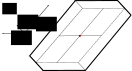
\includegraphics[width=0.5\linewidth]{graphics/zonotope}
  \captionof{figure}{Exemplary creation of a Zonotope $Z$ with $d=2$, $k=3$ and the three generators $p_1,p_2,p_3$.}
  \label{fig:zonotope}
\end{figure}

\end{definition}

When applying the projection $W_r^T$ to the inputs $x \in \Omega$, it can be seen that it holds:
\begin{equation}
\begin{split}
W_r^T x=~&W_r^T \sum_{i=1}^d x_i e_i\\
=~&\sum_{i=1}^d x_i p_i , ~~~~ p_i=W_r^T e_i
\end{split}
\end{equation}
Therefore, since $x_i \in [0,1]$
\begin{equation}
\{W_r^T x \mid x \in \Omega\}=\left\{\sum_{i=1}^d x_i p_i \mid x \in \Omega \right\}=\left\{ \sum_{i=1}^r x_i p_i \mid 0 \leq x_i \leq 1\right\}
\end{equation}

To get closer to the zonotope definition \ref{zonotope}, we first center the inputs $x \in \Omega$ before applying the projection and divide the generators $p_i$ by 2:
\begin{equation}
\begin{split}
&\left\{W_r^T (x - c_d) \mid x \in \Omega\right\}\\
=&\left\{\sum_{i=1}^d (x_i - \frac{1}{2}) p_i' \mid x \in \Omega \right\}, ~~ p_i'=W_r^T e_i\\
=&\left\{\sum_{i=1}^d (x_i' - \frac{1}{2}) p_i' \mid 0 \leq x_i \leq 1 \right\}\\
=&\left\{\sum_{i=1}^d (x_i' - \frac{1}{2}) p_i' \mid 0 \leq x_i \leq 1 \right\}, ~~ p_i=\frac{1}{2} p_i'\\
=&\left\{\sum_{i=1}^d x_i p_i' \mid -1 \leq x_i \leq 1 \right\}
\end{split}
\end{equation}

Therefore we define
\begin{equation}
p \colon \Omega \mapsto Z, ~~ p(x)=W_r^T (x-c_d)
\end{equation}
and
\begin{equation}
Z=\{\sum_{i=1}^d p_i x_i , ~ -1 \leq x_i \leq 1\}, ~~ p_i=\frac{1}{2} W_r^T e_i
\end{equation}

Then $Z=p(\Omega)$.

\subsection{Surrogate space}

However since the surrogate creation process expects inputs from a $r$-dimensional unit hypercube $\Omega_R$, during the normalization step, the zonotope $Z$ is first encased in an $r$-dimensional hypercube called the surrogate space $S$ which is then scaled and aligned to obtain the unit hypercube $\Omega_r$.
To make the generation of the surrogate space easier, the generators $p_i$ are ordered by their magnitude.
\todo{inwiefern wird es dadurch easier?}

The generators $q_1, \dots, q_r$ of the encasing hypercube are calculated by applying the Gram–Schmidt process on the ordered zonotope genrators $p_i$ with
\begin{equation}
q_i=p_i - \sum_{k=1}^{i-1} \frac{\langle q_k, p_k\rangle}{\langle q_k, q_k\rangle}
\nonumber
\end{equation}

The surrogate space $S$, which encases the zonotope $Z$, is then an $r$-dimensional hypercube with
\begin{equation}
S=\{\sum_{i=1}^r q_i x_i s_i , ~ -1 \leq x_i \leq 1\},~~ s_i=\sum_{k=1}^d \langle q_i, p_k\rangle
\label{surrogate_space}
\end{equation}
where the scaling factors $s_i$ make the hypercube $S$ exactly match the extent of the zonotope $Z$ as shown in \ref{fig:surrogate_space}.


\begin{figure}[H]
\centering
  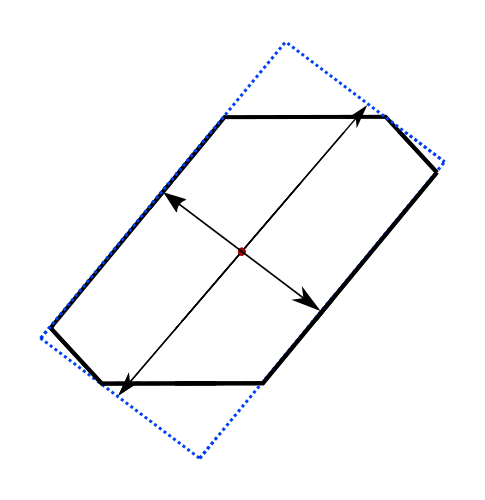
\includegraphics[width=0.4\linewidth]{graphics/s}
  \captionof{figure}{Construction of the surrogate space $S$ for the zonotope of figure \ref{fig:zonotope} according to \eqref{surrogate_space}.}
  \label{fig:surrogate_space}
\end{figure}

In theory, the generators $p_i$ that are used to calculate the $q_i$ don't have to be ordered.
However, to improve the generation of the surrogate space, the generators $p_i$ are ordered by their magnitude w.l.og. $|p_1|\geq \dots \geq |p_d|$.
This will improve the surrogate space $S$ in terms of unused space $S \setminus Z$.
\todo{Proove?}


\subsection{Reduced unit hypercube}

The surrogate space $S$ can then be easiliy transformed into a unit hypercube $\Omega_R$ as shown in \ref{fig:aligned} and therefore elements $z \in Z$.
First, by using a change of basis from the unit basis into the surrogate space basis given by the $q_i$.

Let
\begin{equation}
Q=\begin{bmatrix}
  \\
    q_1 ~ q_2 ~ \dots ~q_{r-1} ~ q_r\\
    \\
  \end{bmatrix}
  , ~~
\label{alignment}
\end{equation}
be the new basis matrix.

We can then obtain $u=Q^T z$, where $u_i \in [-s_i,s_i]$ since this is the range of the surrogate space defined in \ref{surrogate_space}.
Once the projected inputs $z \in Z=p(\Omega)$ are represented by the new basis, it is trivial to transform the surrogate space into an $r$-dimensional unit hypercube $\Omega_r$.
First, the $u$ have to be scaled down with
\begin{equation}
u_s=\Gamma u, ~~ \Gamma=\text{diag}(\frac{1}{2 s_1}, \dots, \frac{1}{2 s_r}), ~~
\label{alignment}
\end{equation}
s.t. $(u_s)_i \in [\frac{1}{2},\frac{1}{2}]$.

Then the $u_s$ just have to be translated again from the center away with
\begin{equation}
t_{\text{Cube}}(x)=c_r + u_s
\end{equation}

\begin{figure}[H]
\centering
  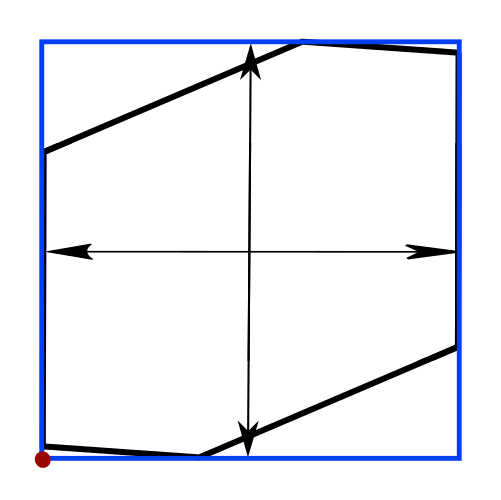
\includegraphics[width=0.4\linewidth]{graphics/s_unit}
  \captionof{figure}{Transformation of $S$ from figure \ref{fig:space} into a unit hypercube according to \eqref{alignment}}
  \label{fig:f2_combined_rel_errors_inter}
\end{figure}


\subsection{Reversing the transformation}

While it is not required to revert the previously shown transformation process, i.e. going from $\Omega_r$ to $\Omega$, later figures in this thesis use the described reversing to illustrate lower dimensional transformed sparse grids in the original and higher-dimensional space.
It is therefore only shown in a more informal way.

\textbf{Inverting the transformation  }
For certain operations it is necessary to invert the transformation.
For this we define the inverse transformation as follows:
\begin{equation}
t^{\text{inv}}(x_{t})=\{x \in \Omega \mid t(x)=x_{t}\}
\end{equation}
In the case of a linear dimensionality preserving transformation, it holds that $|t^{\text{inv}}(x_{t})| \in \{0,1\}$.
Otherwise, we can't infer anything about the cardinality of the inverse, i.e. $|t^{\text{inv}}(x_{t})| \geq 0$.
Luckily there is no need to compute $t^{\text{inv}}(x_{t})$. Instead for conducting operations on the surrogate, it suffices to determine wether a point $x_t \in \Omega_t$ is unused, i.e. $|t^{\text{inv}}(x_{t})| = 0$, which can be done quickly.
\\
\\

Let $y=t_{\text{Cube}}(x)$ be the transformed input. It then holds that
\begin{equation}
x=(W_r Q \Gamma^{-1} (y - c_r)) + c_d
\end{equation}

\section{Active Subspaces}


The method of active subspaces \cite{CG15} aims to identify the most influential directions in the parameter space to construct a lower-dimensional subspace of $\Omega$ which covers most of a models output variance to conduct parameter studies with a reduced amount of dimensions.
In constrast to conducting parameter studies, we will use the so-called active directions to construct the $W_r$.
Let
\begin{equation}
C = \int_{\Omega} (\nabla f) (\nabla f)^T \rho ~ dx
\label{as_c}
\end{equation}
be the average outer product of the gradient, a $(d \times d)$ matrix.
Since $C$ is a positive semi-definite matrix, it is possible to decompose it into its eigenvectors $v_i$ and their corresponding real eigenvalues $\lambda_i$ with
\begin{equation}
C = V \Lambda V^T, ~~ \Lambda = diag(\lambda_1, ..., \lambda_d), ~~ V=
  \begin{bmatrix}
  \\
    v_1 ~ v_2 ~ \dots ~ v_{d-1} ~ v_d\\
    \\
  \end{bmatrix}
\nonumber
\end{equation}

We furthermore assume that the eigenvectors in this decomposition are ordered, i.e. $\lambda_1 \geq ... \geq \lambda_d$.
A larger eigenvalue indicates a higher rate of change along the direction, more precisely it is the average squared directional derivative of f with respect to its eigenvector $v_i$ \cite{CG14} with
\begin{equation}
\lambda_i=\mathds{E}[((\nabla f)^T v_i)^2]
\label{eigenvalues}
\end{equation}
Therefore, the column vectors of the matrix $V$ are ordered from most the active direction $v_1$ to least the active direction $v_d$.
By keeping only a specific amount of the most active directions $r \leq d$ we obtain
\begin{equation}
W_r=\begin{bmatrix}
  \\
    v_1 ~ v_2 ~ \dots ~ v_{i-1} ~ v_r\\
    \\
  \end{bmatrix}
\label{basis}
\end{equation}

In the context of this thesis, the given input sample $S$ is used to derive the matrix $C$ from \ref{as_c} using a classical Monte-Carlo approach.
The matrix $C$ can then be approximated with
\begin{equation}
C \approx \frac{1}{n} \sum_{i=1}^n  (\nabla f(y_i)) (\nabla f(y_i))^T
\nonumber
\end{equation}




\subsection{Estimating gradients}

If the gradient function is not known and can not be calculated analytically, the gradients can be approximated in various ways.
There are various different methods of achieving that, however each method has its advantages and disadvantages as will be showcased in this section.

\begin{definition}[Active Subspace error]
Let $A \in \mathds{R}^{m \times n}$. Then
\begin{equation}
\| A\|_2=\sqrt{\sum_{i=1}^m \sum_{j=1}^n |a_{i,j}|^2}
\nonumber
\end{equation}
is the Frobenius norm of the matrix $A$.
Given an estimated Active Subspace eigenvector matrix $V$ and the reference eigenvector matrix $V^*$, the
Active Subspace error is calculated with
\begin{equation}
e_{\text{AS}}(V)=\| V - V^* \|_2
\nonumber
\end{equation}
\end{definition}

In the context of Active Subspaces, the approximation error of the gradients is not the relevant metric to evaluate a method.
Instead, the primary focus is the Active Subspace approximation error, which is decoupled from the individual gradients, since it is based on the average outer product of the gradients.
While the individual gradients approximated by different methods can be far off, the gradient average can still come close to the real one if the general trend of the gradients is still be reflected with the method.
Therefore, inaccuracies of single gradients can be averaged out but systematic biases of the gradients will influence the Active Subspace.


\subsection{Finite differences}

The most common approach to estimate the gradients are finite differences.
In this thesis, an adaptive mix of forward and backward differences are used with a fixed distance $h$ where the range of possible distance is defined by $0 < h \leq 0.5$ such that
\begin{equation}
\frac{\partial f(x)}{\partial x_i} \approx
\begin{cases}
    \dfrac{f(x_1, \dots, x_i + h, \dots, x_d) - f(x)}{h}, & x_i + h \leq 1 \\[1.5em]
    \dfrac{f(x_1, \dots, x_i - h, \dots, x_d) - f(x)}{h}, & \text{else}
\end{cases}
\end{equation}

The downside in the context of the sample-based approach is the requirement to additionally evaluate the model function at $d$ other inputs to determine the gradient at one sample point.
For high $d$ and a large amount of samples $n$, $dn$ function evaluations for finite differences may become too costly.
Alternatively, the gradients can be determined using a different approach that only works on a given input sample and does not require other function evaluations.

\subsection{Directional derivatives}

Another approach is to roughly approximate the gradient by looking at neighboring points in the same sample and using directional derivatives to create a system of linear equations for the gradient at a certain input.
Given two inputs $x, y \in \Omega, x \neq y$, we define the distance between the two inputs as $d=y-x$ and the direction of the distance as the normalized distance with $r=\frac{d}{|d|}$.
By extrapolating the gradient along the direction, we can define an approximation rule with
\begin{equation}
d (\nabla_x f) \approx f(y) - f(x)
\end{equation}

Using $m \in \mathds{N}$ neighbours of a sample point $x \in \Omega$ with $y_i \in \Omega \setminus \{x\}, ~ i \in \{1, \dots, m\}$, we can create a system of linear equations with
\begin{equation}
\begin{bmatrix}
    y_1 - x\\
    \vdots \\
    y_m - x
  \end{bmatrix}  \nabla_x f =\begin{bmatrix}
    f(y_1) - f(x) \\ \vdots \\  f(y_m) - f(x)
    \\
  \end{bmatrix}
  \label{dd_sle}
\end{equation}

One limitation of this calculation is the linear nature of the calculated gradients, i.e. estimating gradients of a non-linear function can lead to biased gradients.
Furthermore, the choice of the $y_i$ heavily influences the result as well as the size of $m$.
The next sections introduce different ways of selecting the neighbours $y_i$ and also evaluate the results.

\subsection{Random neighbour approximation}

The random neighbour approximation method takes as an input a subsample $S' \subseteq S \setminus \{x\}$ with $|S'|=n' < n$.
The set $S'=\{y_1', \dots, y_{n'}'\}$ is called a random neighbour set of $x$.
This random neighbour set is then used as an input for \ref{dd_sle} to approximate the gradient $\nabla_x f$.
For $n,n' \to \infty$, the approximated gradient does not converge to the actual gradients, since the expected distance to the neighbours in a random neighbour set does not go to zero.

\subsection{Nearest neighbour approximation}

The nearest neighbour variant picks a subset $S' \subseteq S$ with a manageable size $n'=|S'|$ similar the the random neighbour method and then calculates the $m \leq n'$ nearest neighbours $y_1',\dots,y_m' \in S'$ of the point $x$ with $|(y_1'-x)| < |(y_2'-x)|< \dots<|(y_{n'-1}'-x)| < |(y_{n'}'-x)|$.
Compared to the random neighbour approximation, for $n,n',m \to \infty$, the approximated gradient does converge to the actual gradient, since the expected distance to the neighbours does go to zero.

\section{Approximation quality}

To get an idea of the actual quality of the different methods, this section will focus purely on the gradient approximation methods as a ... before the methods are used in the surrogate creation process later on.
Two example functions are investigated with the focus being on first the gradient approximation quality and the subsequent Active Subspace approximation quality.

\newpage

\subsection{Simple function}

\begin{equation}
f_1(x)=(0.8 {x_1}^2 - x_2) / (x_3 + 0.5)
\nonumber
\end{equation}

\begin{figure}[H]
\begin{center}
	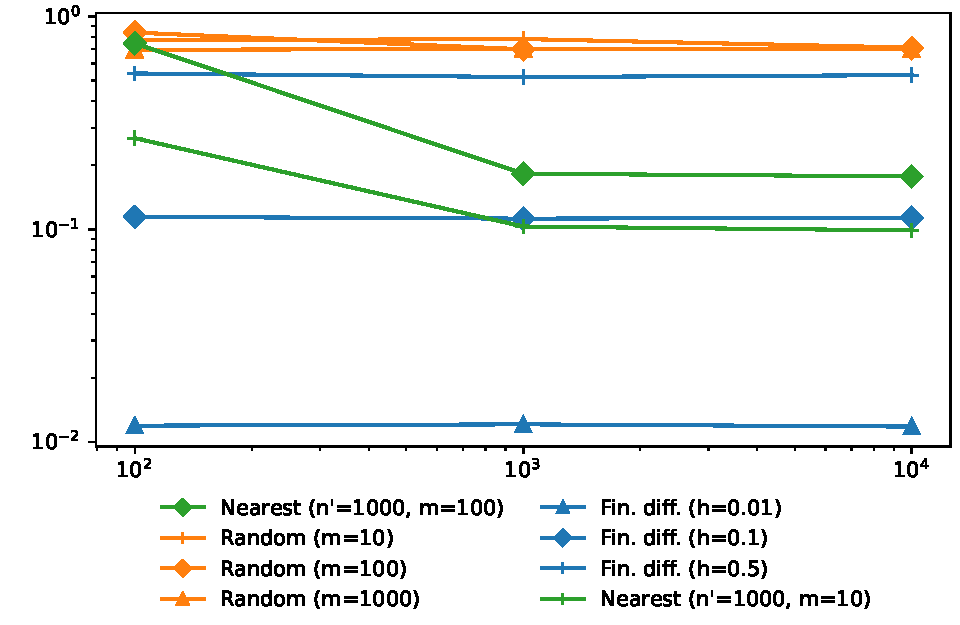
\includegraphics[width=\textwidth]{graphics/as_grad_errors_f1}
\end{center}
	\captionof{figure}{Average $L^2$ error of gradients calculated with the previously introduced methods compared to the actual gradients for $f_1$.}
	\label{fig:as_grad_errors_f1}
\end{figure}

As seen in figure \ref{fig:as_grad_errors_f1}, the finite differences approximation error converges towards zero as the step size goes down as expected.
Furthermore, the nearest neighbour method does deliver better results than the random neighbour method, as it also slowly converges to zero.
The random neighbour methods do not converge but are instead in a range that is even worse compared to the finite differences approximation with a very big step size.

\begin{figure}[H]
\begin{center}
	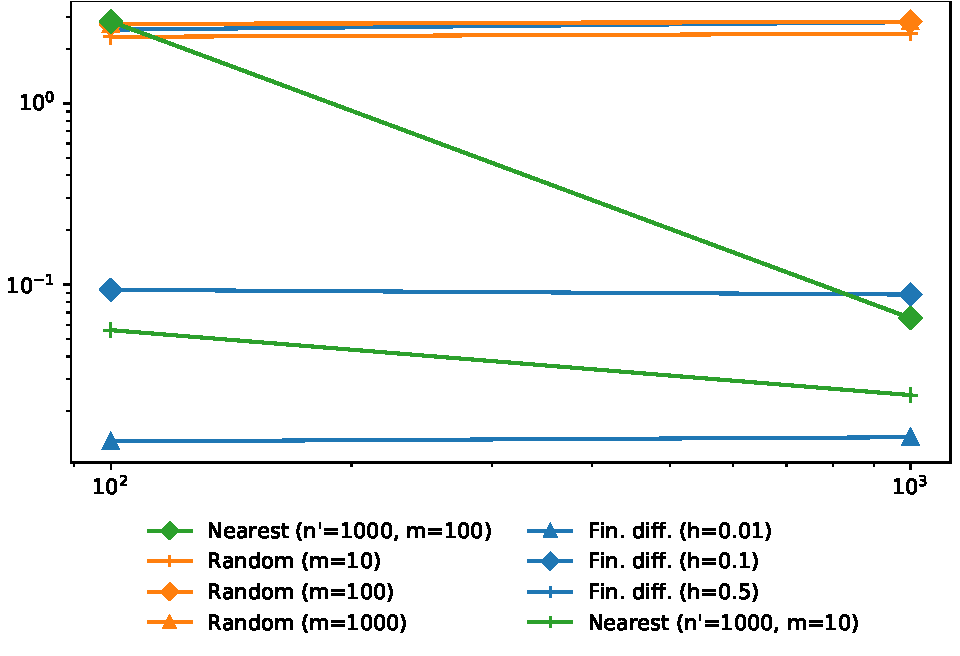
\includegraphics[width=\textwidth]{graphics/as_errors_f1}
\end{center}
	\captionof{figure}{Mean Active Subspace error calculated with the previously introduced methods compared to the actual Active Subspace for $f_1$ over 10 iterations .}
	\label{fig:as_errors_f1}
\end{figure}

As a result of the approximation qualities shown in figure \ref{fig:as_grad_errors_f1}, the gradient approximation qualities behave similar.
The random neighbour methods are still in a small range with an error comparable to the finite differences approximation with a very big step size.
The nearest neighbour method does deliver far better results than the random neighbour method, as it shows a similar quality as the finite differences approximation with smaller step sizes.
Also, using fewer closer neighbours $m$ for the nearest neighbour method seems to be better.

\newpage

\subsection{Complex function}

The second case study is a 20-dimensional function:

\begin{align}
\begin{split}
f_2(x_0, \dots, x_{19})=&e^{0.2 x_0 x_1 x_2 x_3 x_4}\\
+ &5 * sin(\pi x_5 x_6 x_7) x_8^2 x_9^5 x_{10}\\
+ &(x_{11} + 2)^2 x_{12}\\
+ &2 x_{13} * 3 x_{14}\\
+ &x_{15} x_{16}\\
+ &log(1 + (10 x_{17} / (0.1 + x_{18} + x_{19})))
\end{split}
\end{align}

\begin{figure}[H]
\begin{center}
	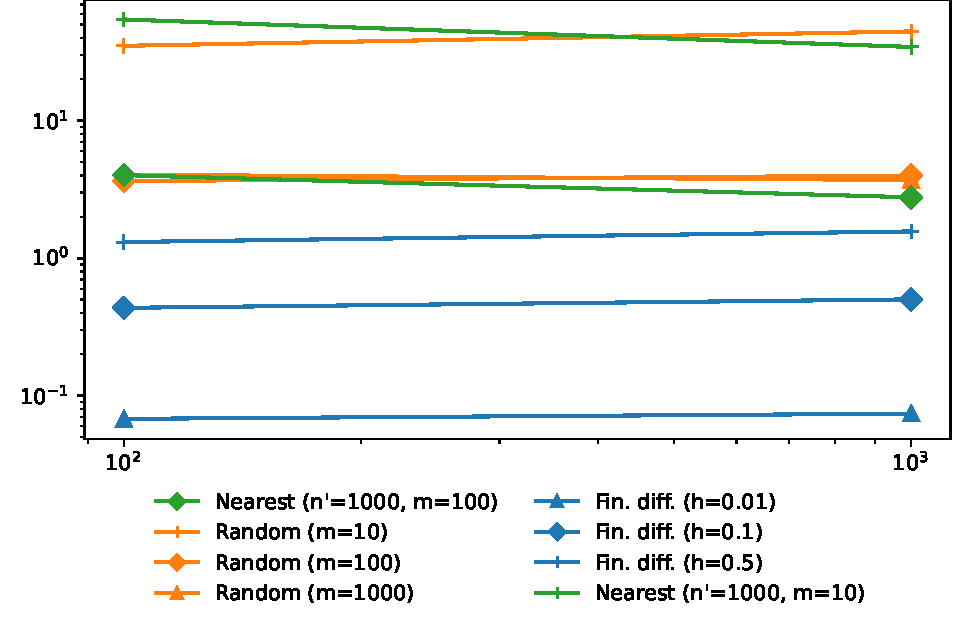
\includegraphics[width=\textwidth]{graphics/as_grad_errors_f2}
\end{center}
	\captionof{figure}{Average $L^2$ error of gradients calculated with the previously introduced methods compared to the actual gradients for $f_2$.}
	\label{fig:as_grad_errors_f2}
\end{figure}

As seen in figure \ref{fig:as_grad_errors_f2}, the finite differences approximation error converges towards zero as the step size goes down as expected.

\begin{figure}[H]
\begin{center}
	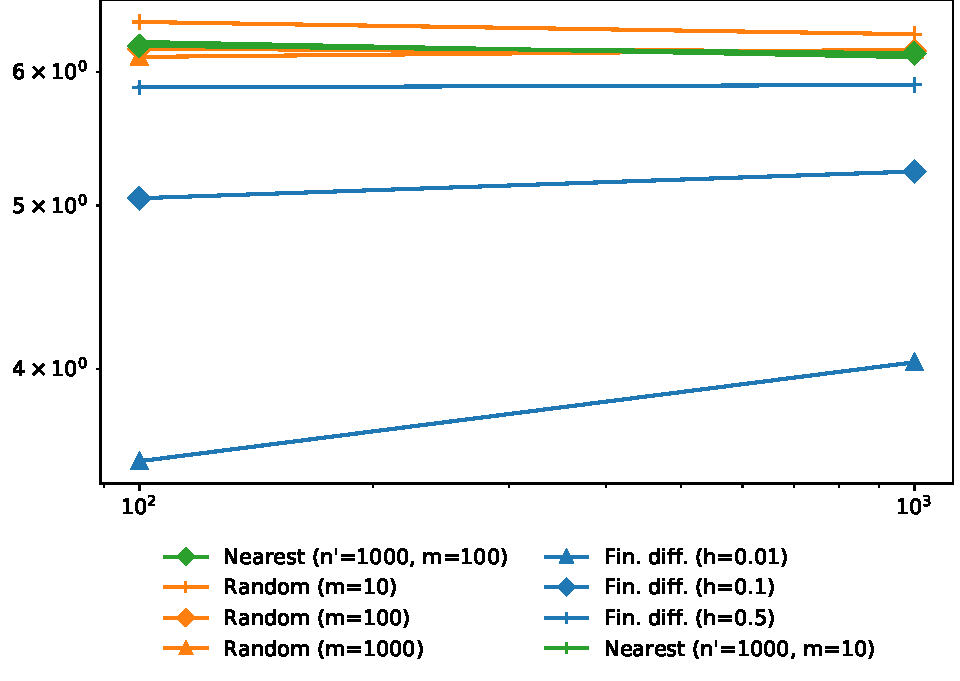
\includegraphics[width=\textwidth]{graphics/as_errors_f2}
\end{center}
	\captionof{figure}{Mean Active Subspace error calculated with the previously introduced methods compared to the actual Active Subspace for $f_2$ over 10 iterations .}
	\label{fig:as_errors_f2}
\end{figure}

...

\section{Random linear transformations}

A completely different approach to finding a transformation function is just generating a random one.
A random transformation generator is easy to implement, can generate new transformation functions almost instantly and offers a purely exploratory approach to finding the best transformation.
It can also serve as a reference for comparision as one would expect that the Active Subspace method should always output better transformation.

As shown in \cite{ABC}, generating uniformly distributed orthonormal matrices is not trivial.
Therefore, this thesis uses the presented algorithm that works like this:
\begin{equation}
z_{i,j} \sim \mathcal{N}\left(0, 1\right)
\end{equation}

The matrix $Z$ is then used in a $QR$ decomposition with $Z=QR$.
The entries diagonal matrix $R$ are then normalized to get
\begin{equation}
\Phi=\text{diag}(\frac{r_{1,1}}{|r_{1,1}|}, \dots, \frac{r_{d,d}}{|r_{d,d}|},)
\end{equation}

The matrix $Q \Phi$ is then uniformly distributed with Haar measure.



\section{Periodic transformations}

Another use case for transformations are periodic functions.
If the model function $f$ is for example periodic along one dimension $i$, i.e. $f(x_1,\dots,x_i,\dots,x_d)=f(x_1,\dots,x_i\text{ mod } h, \dots,x_d)$, we can easiliy define a transformation with $t(x_1,\dots,x_i,\dots,x_d)=(x_1,\dots,(x_i\text{ mod } h) /h, \dots,x_d)^T$ and create a surrogate with $f(x) \approx \hat{f}(t(x))$.
This way, the function can be interpolated better because there are effectively $1 / h$ times more grid points spent along the $i$-th dimension.
Of course this can concept can be expanded upon with multiple periodic dimensions, antiperiodic functions, offsets and combination with linear transformations.

\todo{Example with $f(x)=sin(2\pi x_1) x_2^2$}

\section{Active Manifolds}

Inspired from Active Subspaces, which are purely linear in their nature, one can extend the concept to identifying a one-dimensional curve in the domain $\Omega$ along the flow of most active change, which is called the Active Manifold.
Compared to Active Subspaces, calculating the Active Manifold is more complex and resource intensive.
Furthermore, defining a transformation function that maps from $\Omega$ onto the local one-dimensional space of the curve is way more complex and can be constructed in many ways.
Also they are currently limited to one dimension, for which the surrogate construction method becomes pretty irrelevant.


\chapter{Surrogates for transformations}

Once a transformation function $t(x)$ has been created, the next step is creating a surrogate for the transformed input space $\Omega_r=t(\Omega)$.
The original inputs $y_i \in S$, which were drawn randomly according from the pdf $\rho$, are transformed to obtain the transformed sample $S_r=t(S)$ where the $z_i \in S_r$ transformed inputs with $z_i \in \Omega_r$.
There are many different ways of constructing the surrogate $\hat{f}_r$.
The approach used here is function regression with spatially adaptive sparse grids as described in \cite{P10} where $m \leq n$ samples are used to create an approximation of the model function.
We are aiming to construct the function $\hat{f}_r$ using spatially adaptive sparse grids and an arbitrary basis , i.e.
\begin{equation}
\hat{f}_r(x) \coloneqq \sum_{\underline{l},\underline{i}} \alpha_{\underline{l},\underline{i}} \phi_{\underline{l},\underline{i}}(x)
\end{equation}

The dataset used for the regression is then defined as
\begin{equation}
\{(t(y_i),f(y_i)), ~ y_i \in S, ~ 1 \leq i \leq m\}
\end{equation}
Thus, we are trying to solve the least squares problem with the standard square loss function for the dataset $S$ with
\begin{equation}
\epsilon(\hat{f}_r)=\frac{1}{m} \sum_{i=1}^m (f(y_i) - \hat{f}_r(t(y_i)))^2 
\end{equation}

Note that this data might be, depending on the model to reduce, very noisy and there even might be multiple different values for the same inputs, i.e. $(y_i,f(y_i)), (y_j,f(y_j)) \in S, ~ y_i=y_j, f(y_i) \neq f(y_j)$.
Since the surrogate construction is usually an ill-posed problem and we are calculating a regressed function only based on the samples $S$, the regression method used employs regularization as well to prevent overfitting.
We are therefore solving the regularized least squares problem with the smoothing factor $\lambda > 0$:
\begin{equation}
\hat{f}_r^{\lambda^*} = \argmin_{\hat{f}_r^\lambda \in V} \epsilon_{S}(\hat{f}_r^\lambda) + \lambda R(\hat{f}_r^\lambda)
\end{equation}

\section{Multifidelity surrogates}

The construction of the best possible Sparse Grid surrogate, given inputs, a transformation, and set of possible configuration parameters can become very computationally expensive, since every parameter combination has to be evaluated.
To mitigate this problem, we employ the concept of multifidelity simulations \cite{}, i.e. reducing the cost of parametrization by using low fidelity Sparse Grids and datasets to evaluate a parameter combination and only using high fidelity Sparse Grids and datasets when creating the final surrogate using the determined to be optimal parameters.

A low fidelity Sparse Grid surrogate $\hat{f}^l$ has less grid points compared to an otherwise identical high fidelity Sparse Grid surrogate $\hat{f}^h$.
This means that the level of $\hat{f}^l$ is lower and less or not refinements at all are used.
It is vital that the used low fidelity surrogates still stay representative when comparing the errors for different parameter combinations.
They don't have to be representative of the high fidelity surrogate error, but should fullfil the following property:
\begin{equation}
\epsilon(\hat{f}_1^l) < \epsilon(\hat{f}_2^l) \Rightarrow \epsilon(\hat{f}_1^h) < \epsilon(\hat{f}_2^h)
\end{equation}
i.e. they should be indicative of the comparative quality of their high fidelity surrogates.

This multifidelity approach will also be used in later chapters in a more extended fashion to also evaluate multiple different transformations to choose the best one.
As already mentioned, the ability to evaluate transformations is critical for the random transformation method \ref{}, as it allows for the generation and evaluation of many more transformation to choose the best from.

\section{Operations on transformed surrogates}

Now that a surrogate has been created and we can approximate the model function with $f(x) \approx \hat{f}_r(t(x))$,
we can look at the differences when using transformed surrogates compared to the standard case of directly approximating the model function with $f(x) \approx \hat{f}(x)$ and not using a transformation.

\textbf{Differentiation }
Assuming that the surrogate uses a basis that can be differentiated easily, such as B-Splines, the gradient can be approximated using the chain rule and the gradient function of the transformed surrogate with
\begin{equation}
\nabla f(x) \approx \nabla \hat{f}_t(t(x)) = \nabla (\hat{f}_t \circ t)(x)=(Dt(x))^T \nabla \hat{f}_t(t(x))
\end{equation}
\\
\\
\textbf{Inverting the transformation  }
For certain operations it is necessary to define the inverse of the transformation function.
For this we define the inverse transformation as follows:
\begin{equation}
t^{\text{inv}}(x_{t})=\{x \in \Omega \mid t(x)=x_{t}\}
\end{equation}
In the case of a linear dimensionality preserving transformation, it holds that $|t^{\text{inv}}(x_{t})| \in \{0,1\}$.
Otherwise, we can't infer anything about the cardinality of the inverse, i.e. $|t^{\text{inv}}(x_{t})| \geq 0$.
Luckily there is no need to compute $t^{\text{inv}}(x_{t})$. Instead for conducting operations on the surrogate, it suffices to determine wether a point $x_t \in \Omega_t$ is unused, i.e. $|t^{\text{inv}}(x_{t})| = 0$, which can be done quickly.
\\
\\
\textbf{Transformed distribution}
The input probability distribution $\rho \colon \Omega \to \mathds{R_+}$ with $\int_{\Omega} \rho \; \text{d}x = 1$ also changes for the transformation surrogate.
We define the transformed distribution as
\begin{equation}
\rho_r \colon \Omega_r \to \mathds{R_+}, ~~ \rho_r(x_r)=\int_{t^{\text{inv}}(x_r)} \rho(x) \; \text{d}x 
\end{equation}
This is also a distribution since it holds that
\begin{equation}
\int_{\Omega_r} \rho_r(x_t) \; \text{d}x=\int_{x_r \in \Omega_r} \int_{t^{\text{inv}}(x_r)} \rho(x) \; \text{d}x = \int_{\Omega} \rho(x) \; \text{d}x = 1
\end{equation}
This means that in many cases for example a uniform distribution $\rho$ will be transformed into a non-uniform distribution $\rho_r$.
\\
\\
\textbf{Density Quadrature}
Given an input distribution $\rho$ and transformation $t$, we can compute the integral with
\begin{equation}
\int_{\Omega} f(x) \rho(x) \; \text{d}x \approx \int_{\Omega} \hat{f}_t(t(x)) \rho(x) \; \text{d}x
=
\int_{\Omega_r} \hat{f}_t(z) \left(\int_{t^{\text{inv}}(z)} \rho(x)  \; \text{d}x \right)  \; \text{d}z=
\int_{\Omega_r} \hat{f}_t(z) \rho_t(z) \; \text{d}z
\end{equation}
By introducing a transformation we lose the ability to easily use Sparse Grid based quadrature algorithms.
However, since $r$ is usually smaller than $d$, Monte-Carlo based quadrature becomes a better option for transformed surrogates.
\\
\\
\textbf{Quadrature}
Given a transformation $t$, we can easily compute $\int_{\Omega} f(x) \; \text{d}x$ using the surrogate, since it is a special case of density quadrature with $\rho=\mathcal{U}(0,1)^d$.
Even though the original input is uniformly distributed, the resulting surrogate distribution $\rho_r$ is usually not.
\\
\\
\textbf{Optimization}
To calculate the maximum $x^\text{max} \coloneqq \argmax_{x \in \Omega} f(x)$ or minimum $x^\text{min} \coloneqq \argmin_{x \in \Omega} f(x)$ of the model function, one can also optimize the surrogate. There exist many different algorithms, especially for B-Spline basis functions presented in \cite{}.
After having applied a transformation, there might unused points $x_r \in \Omega_r$ in the surrogate space, i.e. $\nexists x \in \Omega \colon t(x)=x_r$.
Therefore a constrained optimization has to be performed on the surrogate first with
\begin{equation}
x_{r}^\text{max} \coloneqq \argmax_{x_r \in \Omega_r} \hat{f}(x_r), ~ |t^{\text{inv}}(x_{r})|\geq 1
\end{equation}
Afterwards, at least in the dimensionality preserving transformation, we can obtain the maximum $x^\text{max}$ with $x^\text{max}=t^{\text{inv}}(x_{r}^\text{max})$, since $|t^{\text{inv}}(x_{r}^\text{max})|=1$.
One problem is that in the case of a reducing transformation with $r<d$, a computed surrogate maximum $x_{r}^\text{max}$ may be a set of many points.
Therefore another non sparse grid based optimization can be performed on the set $t^{\text{inv}}(x_{r}^\text{max})$, to get a good maximum estimate.

\chapter{Algorithm}

We now covered all the tools needed to approximate the model function with a transformed surrogate.
However, we can take a look at similar methods and take some inspirations from them.
One of these related methods is projection pursuit regression \cite{}.

\section{Projection pursuit regression}

The projection pursuit regression method comes from the area of statistics and is in its core idea related to our approach with linear transformations.
It tries to represent a dataset $P=\{(x_i, y_i)=(x_i, f(x_i))\}$ using the form
\begin{equation}
y_i=\beta_0 + \sum_{i=1}^m f(\beta_i^T x_i) + \epsilon_i
\end{equation}
where $\beta_0$ is a constant, $\beta_i$ are ..., and the $\epsilon_i$ are the residiuals.
Using the $\beta_i$ to project inputs onto a lower-dimensional hyperplane is very similar to our concept of creating linear transformations.


Going from this statistical model to our function approximation problem, we can 
\begin{equation}
f(x)=\sum_{i=1}^m f(\beta_i^T x_i)
\end{equation}
The functions $\hat{f}_i$ and projections $\beta_i$ of this additive model can be calculated iteratively by applying one step of finding a projection and constructing a surrogate repeatedly each time on the error function
\begin{equation}
e_k(x)=f(x) - \sum_{i=1}^k f(\beta_i^T x_i)
\end{equation}

\begin{algorithm}[H]
\normalsize
\begin{algorithmic}
\Function{projectionPursuitRegression}{$f, m$}
    \State $e_0 = f$
    \For{$i = 1, \dots, m$}
    	\State $\beta_i \gets$ best
    	\State $e \gets e_{i - 1} - \hat{f}_i$
    \EndFor
    \State $\hat{f} \gets \sum_{i=1}^m f(\beta_i^T x_i)$
    \State \Return{$\hat{f}$}
\EndFunction
\end{algorithmic}
	\captionof{algorithm}{Pseudocode of the iterative projection pursuit regression algorithm. Alternatively, one could introduce an error exit condition that exists the loop if the regression error is small enough with $\epsilon(e) < \epsilon_{max}$.}
\end{algorithm}

\todo{Mean center function?}

\section{An iterative approach}

\begin{algorithm}[H]
\normalsize
\begin{algorithmic}
\Function{transformedSurrogateSum}{$f, m$}
    \State $e_0 = f$
    \For{$i = 1, \dots, m$}
    	\State $t_i \gets$ generateBestTransformation()
    	\State $\hat{f}_{t_i,i} \gets$ generateBestSurroate($t_i$)
    	\State $e \gets e_{i - 1} - \hat{f}_{t_i,i}$
    \EndFor
    \State $\hat{f} \gets \sum_{i=1}^m \hat{f}_{t_i, i} \circ t_i$
    \State \Return{$\hat{f}$}
\EndFunction
\end{algorithmic}
	\captionof{algorithm}{Pseudocode of the iterative projection pursuit regression algorithm. Alternatively, one could introduce an error exit condition that exists the loop if the regression error is small enough with $\epsilon(e) < \epsilon_{max}$.}
\end{algorithm}

In the case that we use a linear transformation function, the algorithm is pretty much identical to the previous one.

\chapter{Implementation}

To make the shown results as transparent as possible, this chapter will focus on how the previsouly described process of transforming Sparse Grids is actually implemented.

\begin{description}
\item[Object] An object can represent any kind of data, for example a model function, a function sample, a transformation function, a surrogate, and more.
\item[Function] A function takes optional inputs in the form of objects, performs some kind of operation, and outputs an object.
\item[Component] A component is a function declaration, where the actual implementation can be exchanged for many different function implementations.
\item[Control flow + data flow] Arrows signal control flow and also data flow if an object is shown.
\end{description}

\begin{figure}[H]
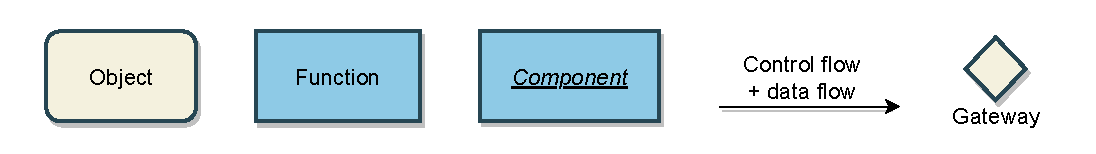
\includegraphics[width=\textwidth]{graphics/definitions.pdf}
\captionof{figure}{Notation used for different elements in the structure diagrams.}
\label{fig:defs}
\end{figure}

Functions and components can also be customized by passing some configuration parameters, which is not explicitly shown in the structure diagrams but will be mentioned if it is done.

\newpage
\section{Pipeline}

The whole reduction process is modeled and implemented as a pipeline made up of different components to allow for maximum flexibility.
All components can be exchanged for many different types, where instances of these types can also be customized by passing some configuration parameters.

\begin{figure}[H]

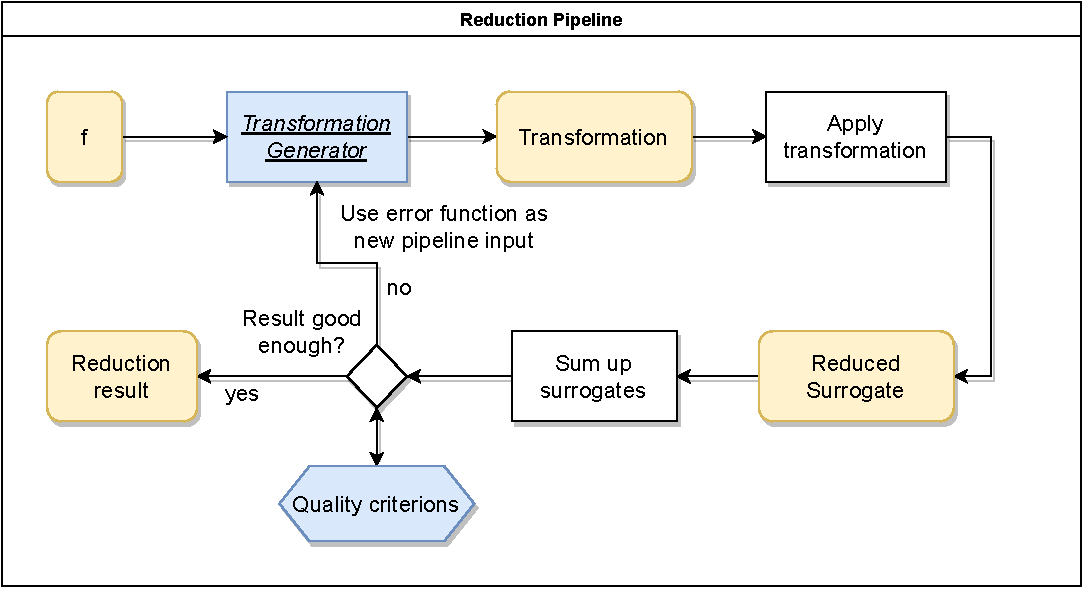
\includegraphics[width=\textwidth]{graphics/ReductionPipeline.pdf}
\vspace{-1.5mm}

\begin{mdframed}[linewidth=0.7px]

\begin{description}
\item[Parameters] {~ \begin{enumerate}[\indent{}]
\item \texttt{\textbf{numIterations}}: Maximum amount of iterations
\item \texttt{\textbf{functionSample}}: A sample
\end{enumerate}}
\end{description}

\end{mdframed}
\captionof{figure}{Component structure of the transformation pipeline and the associated possible configuration options.}
\label{fig:astsg}
\end{figure}

The core component of the reduction pipeline and also the most important one wrt. achieving good reduction results in the transformation function generator.

\newpage
\section {Transformation generators}
\label{sec:tg}

The transformation generator component has the responsibility of finding a good transformation function to use for a pipeline iteration.

\subsection {Transformation stream generator}

Chapter \ref{} covered the used transformation generation methods in detail.
It described that for every calculated Active Subspace matrix or random orthogonal basis, family of transformations can be generated from them, usually accomplished by using different values for the reduced dimension $r$, i.e. cutting less or more dimensions off.
To apply this concept and couple it with other components, such as transformation evaluators, this implementation makes use of so-called transformation generator streams.
A transformation stream generator will generate as much different transformations as it can, where the range of possible transformations is defined by multiple specific parameters.
It can be parallelized.
Every transformation that is generated from the stream is evaluated using a transformation evaluator and the best transformation will be chosen and returned in the end.

\begin{figure}[H]
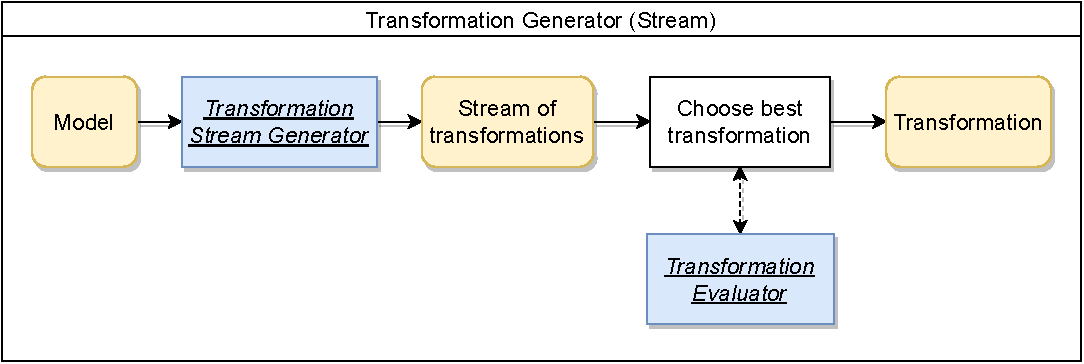
\includegraphics[width=\textwidth]{graphics/TransformationGen_Stream.pdf}
\captionof{figure}{Component structure of a stream-based transformation generator and the associated possible configuration options.}
\end{figure}

\newpage

\subsection{Active Subpsace stream generator}

The already described Monte-Carlo Active Subspace method presented in \ref{sec:as} is implemented as a transformation stream generator component as seen in figure \ref{fig:astsg} , since there are multiple different cutoff possibilities.
The exact range of the cutoff dimensions can be customized using various parameters as seen in figure \ref{fig:astsg}.

\begin{figure}[H]

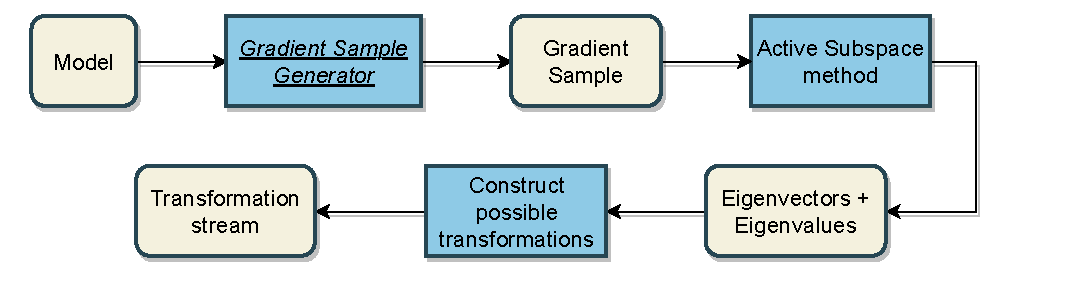
\includegraphics[width=\textwidth]{graphics/TransformationStreamGen_AS.pdf}

\vspace{-1.5mm}

\begin{mdframed}[linewidth=0.7px]

\begin{description}
\item[Parameters] {~ \begin{enumerate}[\indent{}]
\item \texttt{\textbf{maxSampleCount}}: The maximum amount of samples used to create a gradient sample and that is subsequentially passed down to create the Active Subspaces.
\item \texttt{\textbf{minDimensions}}: The minimum amount of used eigen vectors, i.e. the lower bound for $r$.
\item \texttt{\textbf{maxDimensions}}: The maximum amount of used eigen vectors, i.e. the upper bound for $r$.
\item \texttt{\textbf{minEigenValueShare (= 0)}}: Defines a lower bound on the possible values of $r$ by requiring that it holds that $\sum_{i=1}^r \lambda_i / \sum_{i=1}^d \lambda_i \geq \texttt{minEigenValueShare}$.
\end{enumerate}}
\end{description}

\end{mdframed}
\captionof{figure}{Component structure of an Active Subspace transformation stream generator and the associated possible configuration options.}
\label{fig:astsg}
\end{figure}

The Monte-Carlo Active Subspace method requires gradient samples as inputs.
So for a gradient sample generator, four variants can be chosen depending on given inputs and requirements:
\begin{description}
\item[\texttt{\textbf{givenGradient()}}:] If the gradient function of the model function $f$ is known or easy to calculate analytically, then generating a gradient sample is straightforward by just evaluating the gradient function at the sample points.
\item[\texttt{\textbf{finiteDifferences($h$)}}:] Alternatively, the sample gradients can be determined using finite differences if the runtime cost of $d$ model function evaluations per sample point is acceptable.
\item[\texttt{\textbf{randomNeighbour($n'$)}}] Random neighbour approximation according to \ref{}.
\item[\texttt{\textbf{nearestNeighbour($n', m$)}}] Nearest neighbour approximation according to \ref{}.
\end{description}

\newpage

\subsection {Random stream generator}

A completely different approach to finding a transformation function is just generating a random one.
A random transformation generator is easy to implement, can generate new transformation functions almost instantly and offers a purely exploratory approach to finding the best transformation.
It can also serve as a reference for comparision as one would expect that the Active Subspace method should always output better transformation.

\begin{figure}[H]

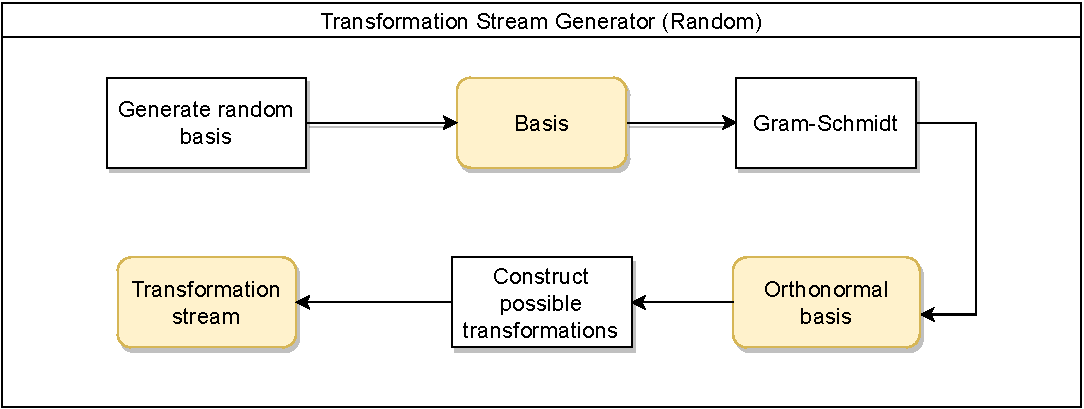
\includegraphics[width=\textwidth]{graphics/TransformationStreamGen_Random.pdf}

\vspace{-1.5mm}

\begin{mdframed}[linewidth=0.7px]

\begin{description}
\item[Parameters] {~ \begin{enumerate}[\indent{}]
\item \texttt{\textbf{minDimensions}}: The minimum amount of used basis vectors, i.e. the lower bound for $r$.
\item \texttt{\textbf{maxDimensions}}: The maximum amount of used basis vectors, i.e. the upper bound for $r$.
\end{enumerate}}
\end{description}

\end{mdframed}
\captionof{figure}{Component structure of an random transformation stream generator and the associated possible configuration options.}
\label{fig:rtsg}
\end{figure}

\newpage

\subsection {Iterative transformation generator}

In some cases, especially when dealing with a random transformation generation as shown in \ref{sec:rtg}, the probability of finding a good transformation in one try is very low, it makes sense to also introduce an iterative transformation generator component, which can be combined with any other transformation generator component, e.g. a stream-based one.
It can therefore also be used with the Active Subspace transformation generator to try to find the best transformation out of several Active Subspace calculations with different input samples.

\begin{figure}[H]
	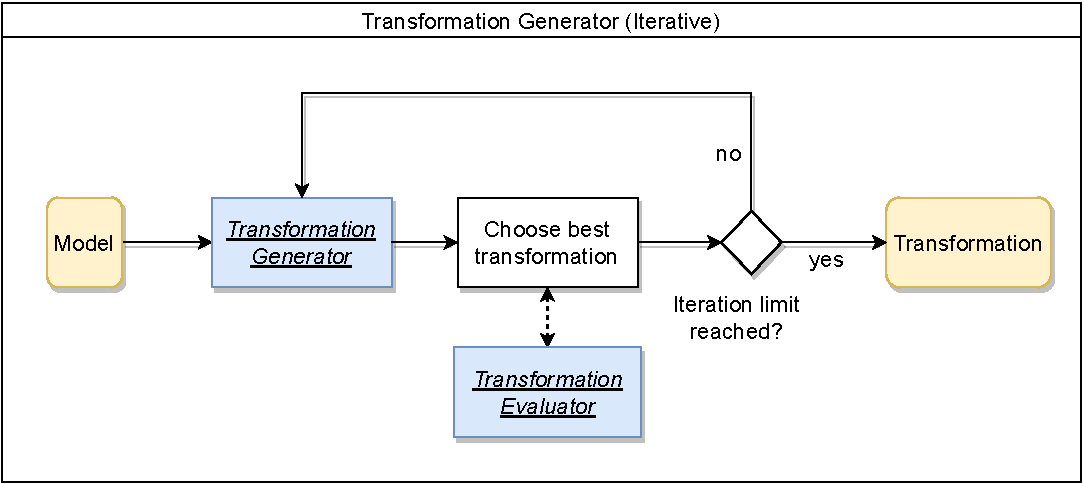
\includegraphics[width=\textwidth]{graphics/TransformationGen_Iterative.pdf}

\vspace{-1.5mm}

\begin{mdframed}[linewidth=0.7px]

\begin{description}
\item[Parameters] {~ \begin{enumerate}[\indent{}]
\item \texttt{\textbf{numIterations}}: Iterative transformation generator configuration options
\end{enumerate}}
\end{description}

\end{mdframed}
\captionof{figure}{Component structure of an iterative transformation generator and the associated possible configuration options}
\end{figure}

\newpage
\section {Evaluators}

\subsection {Surrogate evaluator}

The role of a transformation evaluator is to take a newly constructed transformation $t(x)$, evaluate its quality and make it comparable to other transformations.
This is used for iterative and stream-based transformation generators and by the pipeline.
While this is a pretty straightforward process, it can still be customized by changing the surrogate construction rules and error metric.

\begin{figure}[H]
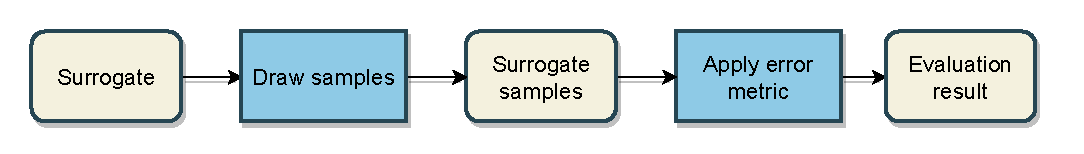
\includegraphics[width=\textwidth]{graphics/SurrogateEval.pdf}
\vspace{-4.5mm}
\begin{mdframed}[linewidth=0.7px]
\begin{description}
\item[\texttt{\textbf{errorMetric}}:] Common error metrics used in this thesis include MSE, RMSE, and NRMSE.
Additionally, penalty terms for various features can be introduced, such as a penalty term that grows with the amount of reduced dimensions of the transformation.
\end{description}
\end{mdframed}
\end{figure}

\subsection {Transformation evaluator}

The role of a transformation evaluator is to take a newly constructed transformation $t(x)$, evaluate its quality and make it comparable to other transformations.
This is used for iterative and stream-based transformation generators and by the pipeline.
While this is a pretty straightforward process, it can still be customized by changing the surrogate construction rules and error metric.

\begin{figure}[H]
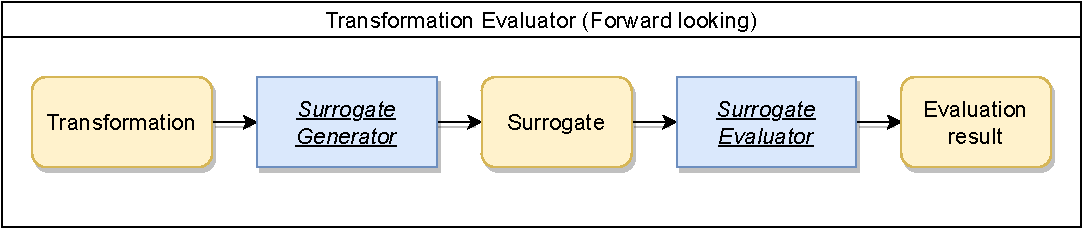
\includegraphics[width=\textwidth]{graphics/TransformationEval.pdf}
\vspace{-1.5mm}
\end{figure}

\newpage
\section {Surrogate generator}

The role of a transformation evaluator is to take a newly constructed transformation $t(x)$, evaluate its quality and make it comparable to other transformations.
This is used for iterative and stream-based transformation generators and by the pipeline.
While this is a pretty straightforward process, it can still be customized by changing the surrogate construction rules and error metric.


\subsection {Sparse Grid surrogate generator}

In the case of Sparse Grid surrogates, as used in this thesis, the construction parameters contain all required inputs like grid type, basis functions, level, adaptivity properties, and more.
As runtime performance is important, especially when using evaluators with the iterative transformation generator, finding the right Sparse Grid level ...

\begin{mdframed}[linewidth=0.7px]
\begin{description}
\item[Parameters] {~ \begin{enumerate}[\indent{}]
\item \texttt{\textbf{gridType}}: Type of basis functions according to \ref{}
\item \texttt{\textbf{basisType}}: Type of basis functions according to \ref{}
\item \texttt{\textbf{approxGridPoints}}: Type of basis functions according to \ref{}
\item \texttt{\textbf{maxTrainSamples}}: Type of basis functions according to \ref{}
\item \texttt{\textbf{trainData}}: Type of basis functions according to \ref{}
\item \texttt{\textbf{lambdas}}: Type of basis functions according to \ref{}
\item \texttt{\textbf{refinements}}: Type of basis functions according to \ref{}
\end{enumerate}}
\end{description}
\end{mdframed}

\subsection {RBF surrogate generator}

\chapter{Implementation and evaluation}

The goal is to answer the following questions:

\begin{enumerate}
\item What is a good amount of samples? How do different sampling techniques influence the results?

\item How good is the quality of the computed $A_k$ for a certain amount of samples? We compare the errors that occur when using the optimal $A_k$ and the computed $A_k$.

\item How much does a certain deviation of the $A_k$ effect the interpolation error?

\item How much do more iterations influence the resultung errors?

\item Is there a local or global convergence for the iterative algorithm? What happens to the convergence error value if we introduce a wrong $A_k$ during a step?

\item How well does the method handle unused dimensions and noise? We inspect the errors for a different amount of unused inputs and varying noise intensity.

\item How high can the input dimension be? In theory, the input dimension can rise arbitrarily high as long as the effective dimensionality does not change. However, at some point the amount of samples used to construct the Active Subspace must be too low for accurate results.

\item What is the best way of determining the amount of reduced dimensions $r$ during each step that leads to the best result? How well suited are the eigenvalues of the Active Subspace for this task?
\end{enumerate}

Every question will be answered by looking at one or more example functions or datasets.

\chapter{Automatic configurations}

As shown in the previous chapters, there are a lot of configuration options for the complete reduction pipeline.
The goal in this chapter is to provide good default configurations and also an algorithm for automatic configuration generation based on a given model function, using the insights from the previous chapter.

\chapter{Conclusion and outlook}



\appendix
\chapter{Appendix}

\subsection{B-Spline basis}

One downside of the hat basis is that the functions do not have a continuous derivative.
Instead, there are discontinuities at the grid point $x_{l,i}$ itself where the derivative flips its sign and at the neighbouring grid points $x_{l,i+2}$ and $x_{l,i-2}$ where the derivative changes to zero.
One solution to eliminating these discontinuities are B-Splines, which are just piecewise polynomials.
\begin{definition}[B-Splines]
Let $p \in \mathds{N}$.
Then
\begin{equation}
b^0(x) \coloneqq
\begin{cases}
    1, & x \in [0,1) \\
   0, & \text{else}
\end{cases}
\end{equation}
is a B-Spline of degree $0$ and
\begin{equation}
b^p(x) \coloneqq \frac{1}{p} xb^{p-1}(x) + (p + 1 - x) b^{p-1}(x-1) 
\end{equation}
is a B-Spline of degree $p$.
\end{definition}
This definition of B-Splines is based on the Cox-de-Boor recursion.

\begin{definition}[B-Spline basis functions]
Let $l,i \in \mathds{N}_0$.
Then
\begin{equation}
\phi^b_{l,i}(x) \coloneqq b^p \left( 2^l x + \frac{p+1}{2} -i \right)
\end{equation}
is an univariate B-Spline basis function of degree $p$.
\end{definition}

\subsection{Mod B-Spline basis}

\begin{definition}[Knots]
Let $m,p \in \mathds{N}_0$.
We then define
\begin{equation}
\underline{\xi}=(\xi_0, \dots, \xi_{m + p}) \in \mathds{R}^{m + p}, ~~ \xi_0 \leq \dots \leq \xi_{m + p}
\end{equation}
as a sequence of knots.
\end{definition}

\begin{definition}[B-Splines]
Let $p \in \mathds{N}$.
Then
\begin{equation}
b^0_{i,\underline{\xi}}(x) \coloneqq
\begin{cases}
    1, & x \in [\xi_i,x_i] \\
   0, & \text{else}
\end{cases}
\end{equation}
is a B-Spline of degree $0$ and
\begin{equation}
b_{i,\underline{\xi}}^p(x) \coloneqq \frac{x - \xi_i}{\xi_{i + p} - \xi_i} b_{i,\underline{\xi}}^{p-1}(x) + \frac{\xi_{i+p+1} - \xi_i}{\xi_{i + p} - \xi_i} b_{i+1,\underline{\xi}}^{p-1}(x) 
\end{equation}
is a B-Spline of degree $p$.
\end{definition}

\begin{definition}[Mod B-Spline basis functions]
Let
\begin{equation}
\phi_l^p(x) \coloneqq \sum_{i=0}^{\lceil (p+1)/2 \rceil} (i+1) \phi^p_{l,1-k}(x)
\end{equation}
be the boundary...
\begin{equation}
\phi^{p,\text{mod}}_{l,i}(x) \coloneqq
\begin{cases}
1 &, l=1\\
\phi^p_{l}(x)&, l>1, i=1\\
\phi^p_{l}(x)&, l>1, i=2^l - 1\\
\phi_{l,i}(x)&, \text{else}
\end{cases}
\nonumber
\end{equation}
\end{definition}


\subsection{Modified basis functions}

One method of removing the need of using boundary grid points at least to some degree are modified basis functions.
These basis functions do not require grid points at the boundary.
Instead at every grid level, they extrapolate the values at the boundaries from the grid points closest to the boundaries using a special kind of basis function.
Therefore, it is possible to modify any non-boundary basis $\phi_{l,i}$ by defining the modified basis as follows:
\begin{equation}
\phi^{\text{mod}}_{l,i}(x) \coloneqq
\begin{cases}
1 &, l=1\\
\phi^{\text{left}}_{l}(x)&, l>1, i=1\\
\phi^{\text{right}}_{l}(x)&, l>1, i=2^l - 1\\
\phi_{l,i}(x)&, \text{else}
\end{cases}
\nonumber
\end{equation}
where $\phi^{\text{left}}_{l}$ and $\phi^{\text{right}}_{l}$ are the special boundary extrapolation functions.
Usually $\phi^{\text{left}}_{l}$ and $\phi^{\text{right}}_{l}$ are similar with regards to their structure of the normal basis functions $\phi_{l,i}$, e.g. a hat basis is usually modified with special hat functions.






\subsection{Prewavelets}

A wavelet is a function that has wavelike properties usually with some kind of oscillation around zero.
Many types of wavelet functions are used for signal processing applications because they inhibit some advantageous properties.
One of these properties is the orthogonality property with $\langle \phi_{i},\phi_{j} \rangle = 0$ for all wavelets with $i \neq j$.
Furthermore,  the wavelets are usually discretisized, because it is not possible to analyze a signal using an infinite amount of wavelets.
One wavelet basis that is already used with sparse grids is the so-called mexican hat basis presented in \cite{}, which does not fullfil any orthogonality property.
In fact, using a completely orthogonal basis is quite constraining, i.e. it is not easy to construct a usable orthogonal basis for the context of sparse grids.
However, in the context of sparse grid based ANOVA we can also work with a semi-orthogonal wavelet basis, also called a prewavelet basis.

\begin{definition}[Semi-Orthogonality]
Let $m,n \in \mathds{N}_0, m \neq n$ be two different levels and $\phi_{l,i}$ a basis.
We then call this basis semi-orthogonal if
\begin{align}
\begin{split}
&\langle \phi_{m,i},\phi_{n,j} \rangle = 0
\nonumber
\end{split}
\end{align}
\end{definition}

The basis functions that are used in this thesis are prewavelets with boundary support \cite{GO95,HP17}, which are linear combinations of the hierarchical hat functions $\phi_{l,i}^h(x)$ and have the desirable property of being semi-orthogonal.

\begin{definition}[Boundary prewavelet basis]
The first basis functions are defined as
\begin{equation}
\phi^p_{0,0} = 1\\
\phi^p_{0, 1} = -\phi_{0,0} + \phi_{0,1}\\
\phi^p_{1, 1} = -\phi_{1,0} + \phi_{1,1} -\phi_{1,2}
\end{equation}
For $l \geq 2$ the basis function are defined as 
\begin{equation}
\phi^p_{l,i} = \frac{1}{10} \phi_{l,i-2} - \frac{6}{10} \phi_{l,i-1} + \frac{10}{10} \phi_{l,i} - \frac{6}{10} \phi_{l,i+1} + \frac{1}{10} \phi_{l,i+2}
\label{prewavelet_def}
\end{equation}
with the special boundary cases
\begin{equation}
\phi^p_{l,1} = -\frac{12}{10} \phi_{l,0} + \frac{11}{10} \phi_{l,1} - \frac{6}{10} \phi_{l,2} + \frac{1}{10} \phi_{l,3}\\ \phi^p_{l,2^l-1}(x)=\phi^p_{l,1}(1-x)
\end{equation}
\end{definition}
The multivariate basis functions $\phi^p_{\underline{l},\underline{i}}$ are obtained by applying the tensor-product approach to the univariate basis functions $\phi^p_{l,i}$ to get $\phi^p_{\underline{l},\underline{i}} \coloneqq \prod_{t=1}^{d} \phi^p_{l_t,i_t}$.
These also fullfil the semi-orthogonality with $\langle \phi^p_{\underline{l},\underline{i}},\phi^p_{\underline{l'},\underline{i'}} \rangle = 0$ for $\underline{l} \neq \underline{l'}$.

Test

\newpage
\printbibliography


\pagestyle{empty}
\renewcommand*{\chapterpagestyle}{empty}
\Versicherung
\end{document}
